\section{RECOIN: An Image Representation for Organizing an Image}
\label{sec:atomic:fragments}

As Object Proposal (OP) methods have evolved to address the limitations of the bottom-up traditional segmentation paradigm, the representation on which these algorithms operate have not evolved to the same extent. Traditional image representations have been based on grouping pixels into regions or grouping edges into contours. The resulting shapes have then been represented by various region-based or contour-based representations, including the medial axis. The object proposal methods have not followed this dichotomy in representation, since the vast majority of object proposal methods follow a region-based approach of first grouping pixels into superpixels, as represented by a region-adjacency graph (RAG), but fewer approaches follow a contour-based method. 

The basic premise of this thesis is that the operations necessary to organize a set of image pixels into coherent object parts requires an explicit representation of \emph{(i)} contours for contour operations, \emph{(ii)} regions for regional operations, and \emph{(iii)} spatial organization of curves and regions to make explicit curve and region neighbors. We will show that the traditional wisdom about the equivalence and duality of the boundaries of a region-based representation and conversely the interior of a boundary-based representation breaks down when boundaries are partial (not closed silhouettes) and regions are partial (not full objects). This forces a requirement of a simultaneous explicit representation of partial regions, to allow grouping of pixels which can be grouped with some certainty, an explicit representation into partial contours (contour fragments) so that those edges which can safely be grouped into contours can, and to couple these representations and deal with the resulting redundancy in representation. Our approach is then a coupling of a \emph{region-map}, a \emph{boundary-map}, and a spatial organization of each, as represented by a refinement of the medial axis that is known as the shock-graph. The coupled multilayer representation, which we refer to as RECOIN, is key in dealing with partial information, and in transforming subsequent grouping into multiple conflicting hypotheses, which will prove critical in the face of realistic levels of ambiguity and clutter.


%% The majority of object proposal methods still utilize the very popular graph-based segmentation framework, and hence are based on a region-adjacency graph (RAG) representation of pixels or superpixels. This regional representation though overlooks the other signature that objects leave behind in their projection onto the image, namely, silhouette curves. An unorganized set of contours, traditionally ignored in segmentation or object proposal approaches, provides an alternative set of grouping constraints in addition to those pertaining to superpixels or pixels. In addition to the contour content in isolation, the spatial configuration of these contour fragments is very meaningful. This motivates a coupled, layered approach where superpixel-like regions, contour fragments, and spatial arrangements are all represented. The strength of a multi-faceted representation is in building multiple hypotheses, which are critical 


\subsection{Grouping pixels into Regions: SuperPixels}


Object surfaces frequently enjoy a degree of homogeneity when projected onto an image, in contradistinction to regions containing both an object and other objects or background. Following the ancient adage, ``birds of a feather flock together'', pixels are locally grouped when they share some appearance attributes, resulting in a partition of an image into superpixels. These atomic primitives reduce the degrees of freedom by providing a convenient primitive from which image features can be computed, thus greatly reducing the complexity of higher level computer vision tasks. Furthermore, the partition of the image into a set of regions provides a neighborhood structure and each region is enclosed by a set of contours. Using properties of regions as a cue to further grouping of superpixels into object proposals is well-established, while the use of superpixel boundaries for the same purpose faces two fundamental limitations of the representation itself, described below. 



The first major drawback is that superpixel contours serve two distinct roles: portions of contours correspond to real meaningful boundaries, while the remaining portions are simply delimiters of homogeneous patches resulting from the region formation process. Unfortunately, there is no labeling of which of the region boundaries are image cues and which are an artifact of the grouping process. The challenge in reasoning with contour maps arising from a superpixel type representation is this ambiguity: observe in Figure~\ref{fig:sp_probs1} how these non-veridical contours overwhelm true contours and there is no explicit label in the representation to differentiate them. It is evident that adjusting the granularity of superpixels trades off higher recall for lower precision, Figure~\ref{fig:sp_probs1}\textcolor{red}{(g,h)}. The inability to differentiate between real and artificial boundaries, coupled with a secondary effect namely the poor localization of boundaries which arise from region-grouping, limit the use of grouping-based on superpixel boundaries. Traditionally, this is why methods that operate with superpixels exclusively reason with the region while avoiding its boundaries, although some, \eg Sharon \etal ~\cite{Alpert:etal:CVPR07} do use contours for reasoning with them. 


\begin{figure*}[!ht]
  \centering
{\footnotesize\textit{a}}\includegraphics[width=0.31\linewidth]{figs/175083.jpg}
{\footnotesize\textit{b}}\includegraphics[width=0.31\linewidth]{figs/lizard_100_slic.pdf}
{\footnotesize\textit{c}} \includegraphics[width=0.31\linewidth]{figs/lizard_1000_slic.pdf}
{\footnotesize\textit{d}}\includegraphics[width=0.31\linewidth]{figs/lizard_gt.png}
{\footnotesize\textit{e}} \includegraphics[width=0.31\linewidth]{figs/100_tail_analysis.png}
{\footnotesize\textit{f}} \includegraphics[width=0.31\linewidth]{figs/1000_tail_analysis.png}
{\footnotesize\textit{g}}\includegraphics[width=0.34\linewidth]{figs/pr_100_slic.png}
{\footnotesize\textit{h}} \includegraphics[width=0.34\linewidth]{figs/pr_1000_slic.png}
%{\footnotesize\textit{f}} \includegraphics[width=0.32\linewidth]{figs/pr_1000_slic.png}
{\footnotesize\textit{i}} \includegraphics[width=0.24\linewidth]{figs/slic_pr_curve.pdf}
{\footnotesize\textit{j}} \includegraphics[width=0.34\linewidth]{figs/lizard_40_cons.pdf}
{\footnotesize\textit{k}} \includegraphics[width=0.34\linewidth]{figs/lizard_100_cons.pdf}
{\footnotesize\textit{l}} \includegraphics[width=0.24\linewidth]{figs/cons_pr_curve.pdf}
\caption{ \emph{(a)} An image selected from the Berkeley Segmentation Data Set (BSDS500)~\cite{Arbelaez:etal:PAMI11} and the corresponding SLIC~\cite{Achanta:etal:PAMI12} superpixel representation for \emph{(b)} 100 superpixels and \emph{(c)} 1000 superpixels. Two key observations must be made: \emph{(i)} the finer the segmentation, the larger the likelihood that the boundary region include silhouettes of objects and other important image cues, as annotated by the BSDS Ground-Truth Boundaries shown in \emph{(d)}. For example, in a magnified region of the tail the 100-superpixel boundaries do not capture the tail \emph{(e)} but the 1000-superpixel  boundaries include them \emph{(f)}.  \emph{(ii)} The finer the segmentation, the larger the likelihood that the boundary of the superpixel is not a meaningful image curve, with respect to the GT boundaries. This can be easily seen by marking superipixel boundaries that agree with GT boundaries as magenta and the remaining ones as cyan, shown in \emph{(g)} and \emph{(h)} for the 100 and 1000 superpixels of \emph{(b)} and \emph{(e)} respectively. The precision-recall curve \emph{(i)} shows that with a two-pixel tolerance, only up to 70\% of the true boundaries can be recalled and that is at 20\% precision. In contrast, contour fragments extracted at \emph{(j)} 40 contours and \emph{(k)} 100 contours achieve much higher precision \emph{(l)} at comparative levels of recall. }
 \label{fig:sp_probs1}
%\vspace{-0.751cm}
 \end{figure*}

 %% Visually comparing the marked ground-truth boundaries, Figure~\ref{fig:sp_probs1}\textcolor{red}{b}, with the superpixel boundaries we can see the huge number of spurious boundaries.

 %% The ambiguity of which is which severely limits the usefulness of grouping with superpixel contours. 



 %% that enclose a set of regions. We note these boundaries are not contours due to the lack of ordering, but we consider this a trivial issue as ordering can be enforced.
%% In Figure~\ref{fig:sp_probs1} we illustrate this problem with a specific example. In the top row we see a sample image from the 


%% Selected from the  Berkeley Segmentation Data Set (BSDS500)~\cite{Arbelaez:etal:PAMI11} 



%% and its corresponding superpixel map for a hundred, Figure~\ref{fig:sp_probs1}\textcolor{red}{b}, and a thousand, Figure~\ref{fig:sp_probs1}\textcolor{red}{c}, SLIC~\cite{Achanta:etal:PAMI12} superpixels respectively. In both superpixel partitions, we have randomly colored each of the distinct curve fragments. Our goal then is to reason (merge contours, delete contours, \etc) with this set of contours. The difficulty with reasoning with this type of contour map is the computational complexity of dealing with the large amount of non-veridical contours. Visually comparing the marked ground-truth boundaries, Figure~\ref{fig:sp_probs1}\textcolor{red}{b}, with the superpixel boundaries we can see the huge number of spurious boundaries. Focusing on the tail of the lizard, Figure~\ref{fig:sp_probs1}\textcolor{red}{e,f}, we observe that at hundred superpixels the representation is not capturing the pair of red tail curves at all. If we move to a thousand superpixels, the representation better adheres to the natural image boundaries, but still is missing portions of the tail. We can quantify this by adopting the BSDS evaluation to compare the superpixel boundaries versus the ground truth. We can see in the bottom row, that the number of false positives highlighted in \textcolor{cyan}{cyan} is a substantial portion of the total number of superpixel boundaries. As we go from a hundred superpixels to a thousand superpixels we see an increase in recall, but at the expense of a decrease in precision. Again, since we don't know a priori which boundaries are meaningful boundaries and which are simply delimiters of the grouped pixels we would be forced to reason with this large pool of false-positives boundaries. This computational burden can be reduced by utilizing less superpixels but we lose recall. Finally, we can generate a precision/recall (PR) curve by varying the number of superpixels. We notice that depending on the quality of localization, distance from ground-truth, desired superpixels may or may not be able to achieve that.

\begin{figure}[!ht]
  \centering
{\footnotesize\textit{a)}}\includegraphics[width=0.23\linewidth]{figs/55067_00.png}
{\footnotesize\textit{b)}} \includegraphics[width=0.23\linewidth]{figs/mountain_range.pdf}
{\footnotesize\textit{c)}}\includegraphics[width=0.22\linewidth]{figs/sculpture.png}
{\footnotesize\textit{d)}} \includegraphics[width=0.22\linewidth]{figs/sculpture_cons.pdf}
{\footnotesize\textit{e}}\includegraphics[width=0.22\textwidth]{figs/car_contours.pdf}
{\footnotesize\textit{f}}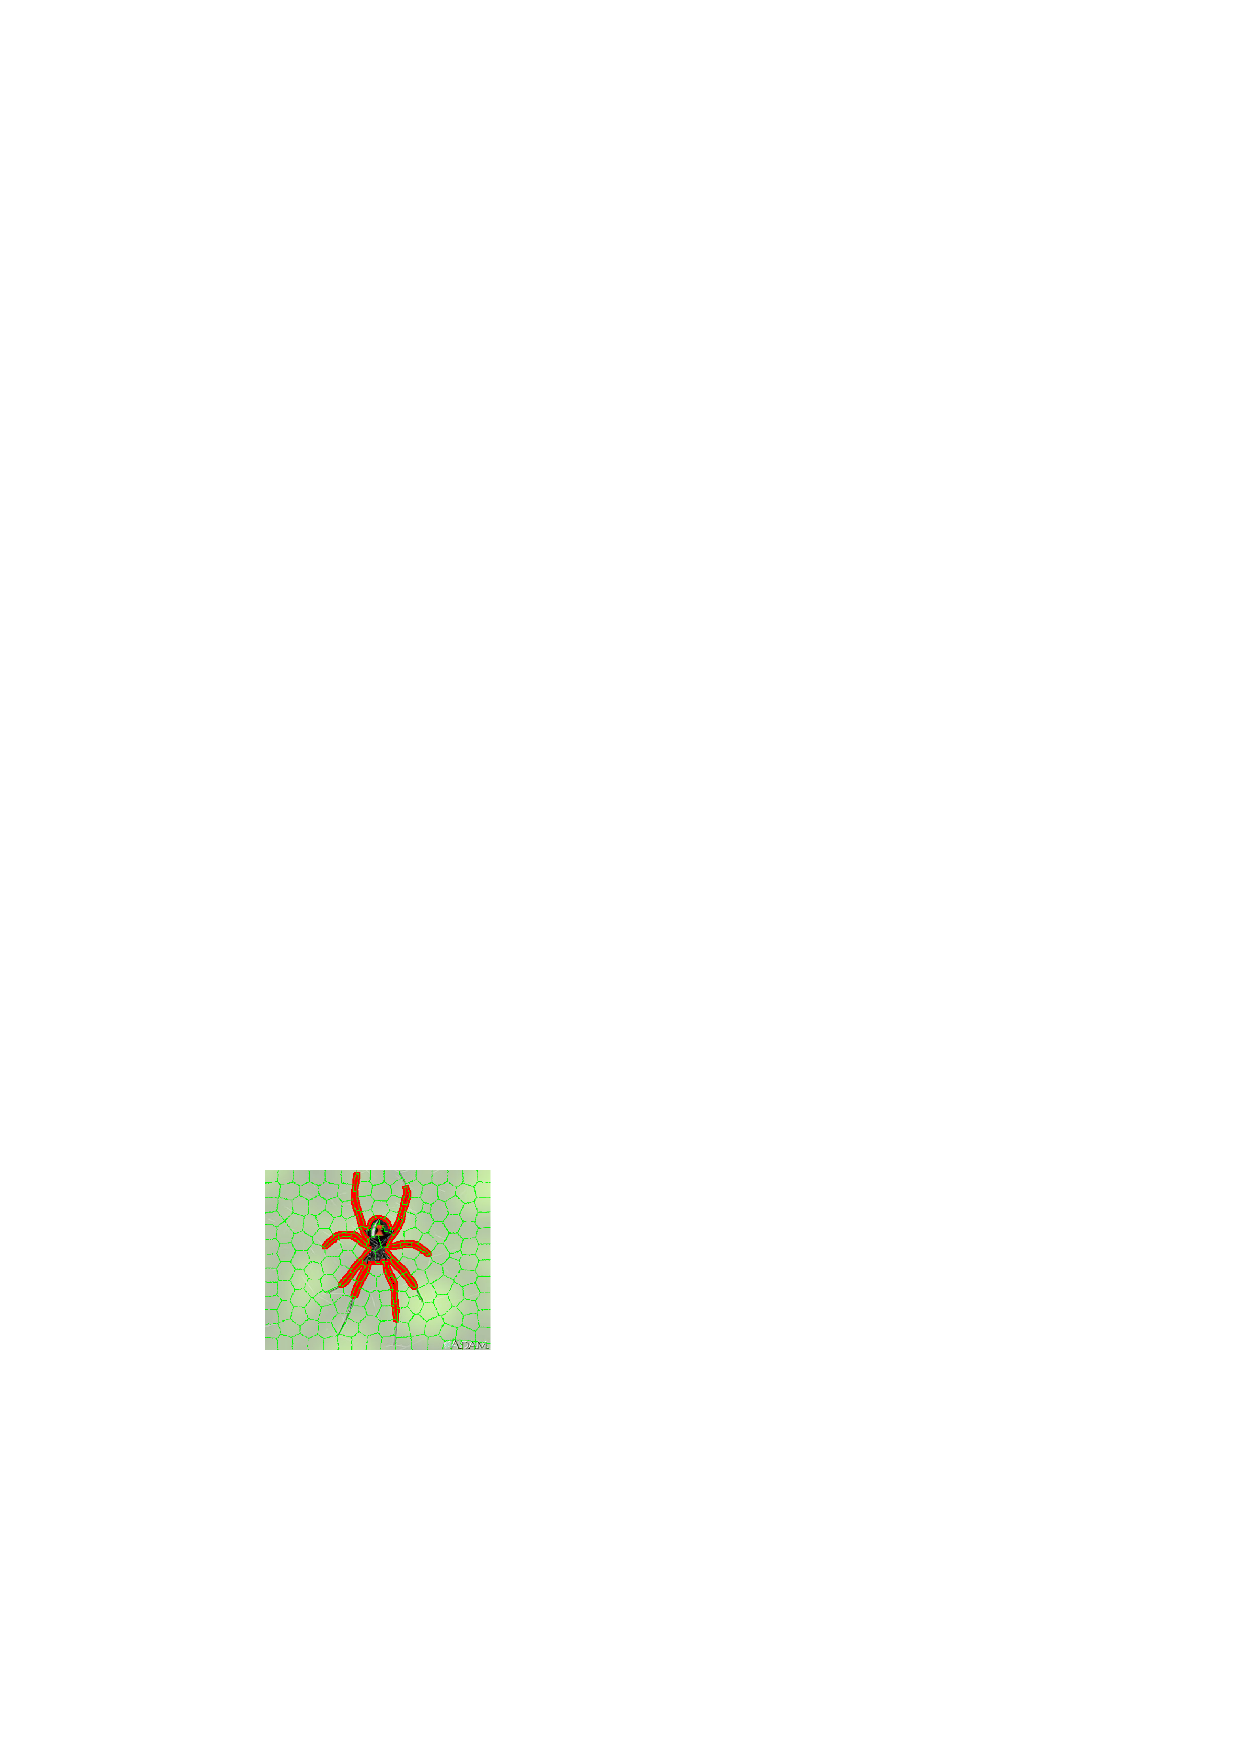
\includegraphics[width=0.22\textwidth]{figs/sp_prob2.pdf}
{\footnotesize\textit{g}}\includegraphics[width=0.22\textwidth]{figs/lizard_tail.pdf}
{\footnotesize\textit{h}}\includegraphics[width=0.22\textwidth]{figs/giraffe_cons.pdf}

\caption{(a) An image of a landscape and in (b) we observe open curves that define the various mountain ranges and tree-line. c) An image of a sculpture and in (d) the various internal open-ended contours that define the structure of the piece. (e) Ground-truth annotations of the car~\cite{Guo:Kimia:POCV12} show that humans perceive all types of contours. f) We show an example from the output of ~\cite{Levinshtein:etal:IJCV12} where all that can be recovered is closed curves. g) The tail (shown in dark pink) of the lizard interacting with the internal contours enclosing each spot create the formation of T-junctions. h) The two contours capturing the silhouette of the giraffe meet at a T-junction. }

%% f) We observe how curves of various configurations are recovered in a contour-based representation of the car.}

 \label{fig:sp_probs2}
%\vspace{-0.751cm}
\end{figure}

The second fundamental difficulty with superpixel contours is due to its construction as the boundary is of closed regions. As such, several types of contours are automatically excluded: \emph{(i)} open contours, as shown in Figure~\ref{fig:sp_probs2}\textcolor{red}{(a-e)} cannot be represented. This is in contrast to the innate capability of such contours to capture closed cues, as exemplified by the approach in~\cite{Levinshtein:etal:IJCV12} where the initial set of disconnected superpixel contour fragments, shown as green in Figure~\ref{fig:sp_probs2}\textcolor{red}{(f)}, merge into a single closed contour by maximizing the appearance difference between background and foreground over the space of all closed curves, Figure~\ref{fig:sp_probs2}\textcolor{red}{(f)}. \emph{(ii)} T-junction where the superpixel contours break the continuous top of ``T'' into two contours with no clear indication as how to recover the grouping of split contours, Figure~\ref{fig:sp_probs2}\textcolor{red}{(g-h)}.  Reasoning with all types of contours namely, closed, open, and junction-forming, requires an augmented representation.  





%% their inability to represent whether individually or grouped the vide variety of contour types. If we look at the human ground-truth markings on the car and tiger, Figure~\ref{fig:sp_probs2}\textcolor{red}{b-d}, we notice that besides the silhouette internal open-ended contours have been delineated along with junction-forming (T,X,Y) contours defined by the interaction of the silhouette with internal markings. If we revisit Figure~\ref{fig:sp_probs1}\textcolor{red}{a-b} we see that each individual superpixel contour is connected to other contours which limits open ended contours and furthermore while junctions bound each superpixel contour it is not clear how to recover contours that form T, Y, or X junctions.  To illustrate this problem we look at a recent paper~\cite{Levinshtein:etal:IJCV12} that advocates for reasoning with superpixel contours. Briefly, this paper groups an 


%% Another fundamental difficulty of superpixels is the inability to represent non-closed regions. To recover non-closed regions and their corresponding boundary requires that the superpixel boundaries need to have a start point and an endpoint \ie an open contour. To illustrate this problem we look at a recent paper~\cite{Levinshtein:etal:IJCV12} that advocates for reasoning with superpixel contours. Briefly, this paper groups a set of disconnected superpixel contour fragments into a single closed contour that maximizes the appearance difference between background and foreground, Figure~\ref{fig:sp_issues}. Observing Figure~\ref{fig:sp_issues} we can see that recovering closed contours amounts to merging 


%%  to organize them into larger closed contours, This brings us to our second drawback of utilizing superpixels is the inability to represent non-closed regions. To recover non-closed regions, such as one leg of the spider of the head of the horse, is even more complicated as it amounts to considering not cycles but all possible paths, blue curve in Figure~\ref{fig:sp_issues}\textcolor{red}{a}, within this graph. This is not only computationally intractable, but also the representation is not amenable to such outputs. 


%% Other strategies include using a coarser number of superpixels or adaptive sized superpixels [Add ref to Chellapa] that lead to less fragmentation. Regardless of approach there will always be some intermingling of veridical and non-sensical boundaries, as region grouping processes are forced to accumulate region information all across the image. The classic example of this is the sky problem where by a large homogeneous portion of the image is artificially broken into many pieces. Even if we adopt an adaptive approach it is unlikely that a superpixel would be of the appropriate size and shape to cover such a large territory. Furthermore, even if we assume these strategies lead to a perfect determination of which boundaries are veridical and which are not, we still would not know which pieces of object boundaries go together. Given that it is unlikely that a single superpixel will cover an object of interest the various delimiters have to be merged similar to an edge linking process or equivalently the consistent regions have to be grouped. In either approach, the output of this process is biased to producing a closed contour. 


 
%% \begin{figure}[ht]
%% \begin{center}
%% {\footnotesize\textit{a}}\includegraphics[width=0.22\textwidth]{figs/sp_prob1.pdf}
%% {\footnotesize\textit{b}}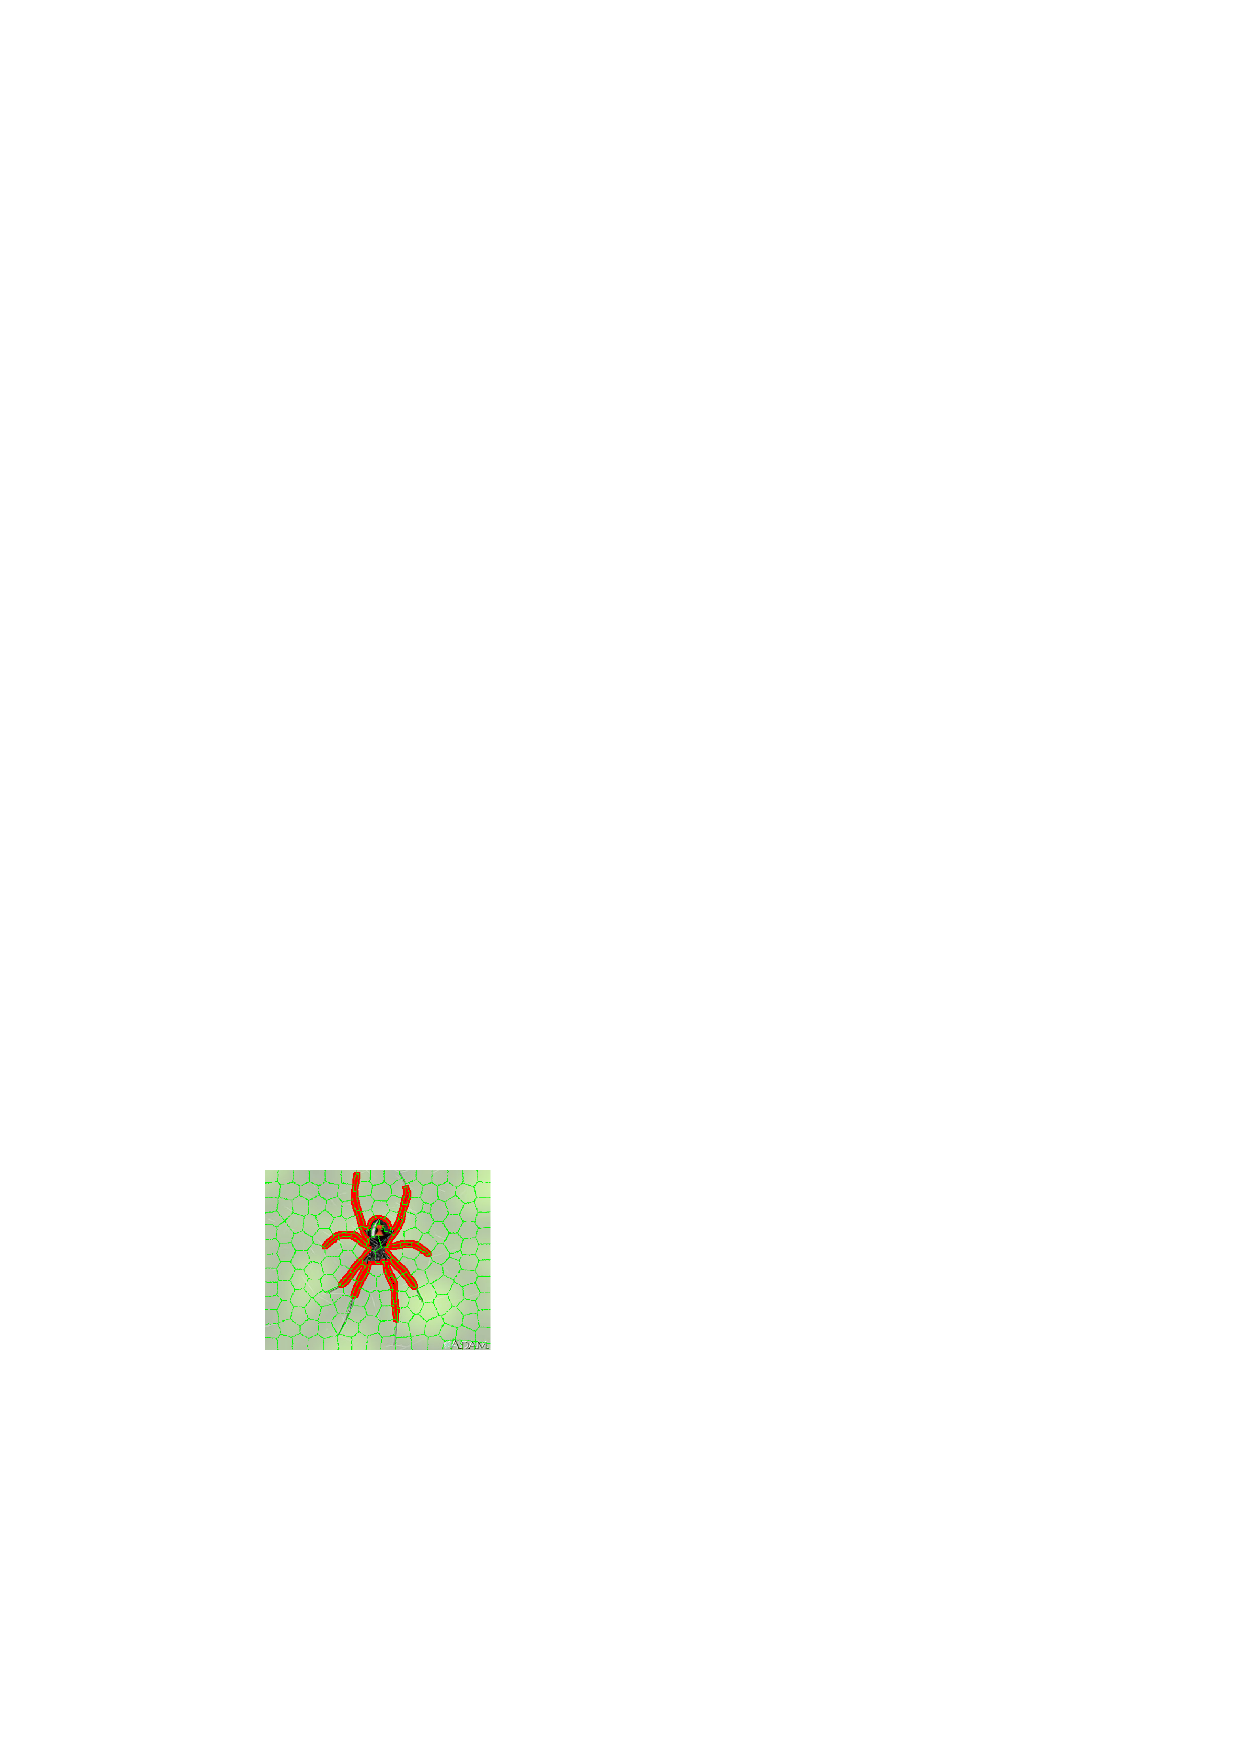
\includegraphics[width=0.22\textwidth]{figs/sp_prob2.pdf}
%% \end{center}
%% \caption{All images courtesy of~\cite{Levinshtein:etal:IJCV12}. a) A small set of superpixels with the red cycle indicating a possible closed contour to consider. The blue path represents the boundary of a non-closed region. b) Examples of a closed boundary recovered using the method of~\cite{Levinshtein:etal:IJCV12}. }
%% \label{fig:sp_issues}
%% \end{figure}

%% Determining the object boundary utilizing superpixels is a difficult task, irregardless of whether the goal is a closed region or not. The task of recovering the contour amounts to merging the various delimiters, which given a superpixel graph amounts to considering all possible cycles~\cite{Levinshtein:etal:IJCV12}, Figure~\ref{fig:sp_issues}. The red-dashed line in Figure~\ref{fig:sp_issues}\textcolor{red}{a} is one possible cycle out of the many combinations that could possibly exist. We can see successful recovery of the closed contour in Figure~\ref{fig:sp_issues}\textcolor{red}{b}, but the subsequent figure depicts an erroneous recovered boundary despite the superpixels perfectly following the silhouette of the horse. 

%% Representing non-closed regions can be not effectively done by a region based description alone. Superpixels and there consistent boundaries can only represent closed curves, 


%% Figures~\ref{fig:sp_probs1}\textcolor{red}{b,c} depict the superpixel boundaries colored in white. If all superpixel boundaries were veridical we would expect the ground-truth pixel map to agree with 



%% Superpixels are perceptually consistent units that adhere well to image boundaries. 

%% serve as the basic unit of reasoning for many region based \emph{object proposal} schemes.


%% They are a compact representation that adhere well to natural image boundaries. Given that each superpixel 


%% As discussed earlier, we would like to reason with types of object signatures: namely regios and contours. One the surface it would seem that superpixels 

%% Superpixels are a popular intermediate from as they capture both regional and contour aspects. 


%% fundamental drawback in using superpixels as an intermediate representation is that 


%% the outer perimeter of each region 

%% They are a compact representation that capture both regional and contour aspects. 

%% Object proposals algorithm generate a wide variety of candidate regions by merging superpixels based on some measure of regional 

%% As discussed earlier grouping methods generate object proposals by merging superpixels based on some notion of regional homenginity. 

%% Superpixels are the basic unit of reasoning about object proposals resulting from grouping pixels into region fragments based on appearance homogeneity. The other signature, though traditionally ignored, of superpixel is the closed boundary that serves as the perimeter of grouped pixels. 

%% enjoy many desirable properties which make them useful for applications even beyond generating object proposals. They are \emph{computational efficient}: the complexity of dealing with hundreds or thousands of pixels in an image is reduced to only a few hundred superpixels. Superpixel maps are \emph{representationally efficient} as pairwise constraints between units, while only for adjacent pixels on the pixel grid, can now model much longer-range interactions between superpixels.  And finally the representation is \emph{near-complete} as there is very little loss in moving from the pixel grid to the superpixel map. 



%% If we look at Figure~\ref{fig:sp_probs1} we see an image 



%% The problem of determining veridical and non-sensical boundaries within a superpixel map is a well known problem. Traditionally this has been dealt with by looking for the presence or absence of contour evidence, predominantly in the form of \emph{Pb} or \emph{gPb} probabilities, for each delimiter. The basis for merging two superpixels, among any other cues, then becomes a function of the contour strength of their separator \emph{i.e} the stronger the evidence the less likely they should be merged as it is indicative of an object boundary. However, while the merging process implicitly considers the type of boundary, this information is not made explicit in the final representation. This subtle distinction makes superpixels inappropriate for our purpose. To illustrate this point, in Figures~\ref{fig:mvf_justify}\textcolor{red}{(a-b)} we see a piece of a horse which is the output of some superpixel merging process and its associated closed boundary. This dual representation of region and boundary is only half correct. While the regional information is highly plausible, the closed contour indicates that this is a whole object rather than a part of something else. What we need is illustrated in Figure~\ref{fig:mvf_justify}\textcolor{red}{c}, where by the closed boundary is split up into a red veridical contour and a blue artificial contour. The superpixel representation is not amenable to such outputs. To recover non-closed regions or parts and their corresponding boundary requires that the delimiters between superpixels need to have a spatial ordering, a start point and endpoint. To call superpixel boundaries as contours is a gross misnomer as they amount to set of unorganized pixels which is sufficient for recovering closed boundaries, but not for non-closed boundaries. Given these drawbacks, the regional representation we desire is one where the true and artificial boundaries are clearly delineated, where each individual boundary is an ordered set of pixels or edges, and finally where each individual boundary's shape and length are maximized to support image evidence. The latter two are precisely what an unorganized set of contours gives us. 
   

%% \begin{figure}[ht]
%% \centering
%% {\footnotesize\textit{a}} \includegraphics[width=0.30\linewidth]{figs/horse_frag_bw.png} 
%% {\footnotesize\textit{b}} \includegraphics[width=0.30\linewidth]{figs/orig_closed.pdf} 
%% {\footnotesize\textit{c}} \includegraphics[width=0.30\linewidth]{figs/orig_actual.pdf}
%% \caption{a) The regional description of a piece of a horse. b) Its associated closed boundary. c) Representing the part by its artificial and real boundaries. }
%% \label{fig:mvf_justify}
%% \end{figure}



%% Other strategies include using a coarser number of superpixels or adaptive sized superpixels [Add ref to Chellapa] that lead to less fragmentation. Regardless of approach there will always be some intermingling of veridical and non-sensical boundaries, as region grouping processes are forced to accumulate region information all across the image. The classic example of this is the sky problem where by a large homogeneous portion of the image is artificially broken into many pieces. Even if we adopt an adaptive approach it is unlikely that a superpixel would be of the appropriate size and shape to cover such a large territory. Furthermore, even if we assume these strategies lead to a perfect determination of which boundaries are veridical and which are not, we still would not know which pieces of object boundaries go together. Given that it is unlikely that a single superpixel will cover an object of interest the various delimiters have to be merged similar to an edge linking process or equivalently the consistent regions have to be grouped. In either approach, the output of this process is biased to producing a closed contour. This brings us to our second drawback of utilizing superpixels is the inability to represent non-closed regions. To recover non-closed regions, such as one leg of the spider of the head of the horse, is even more complicated as it amounts to considering not cycles but all possible paths, blue curve in Figure~\ref{fig:sp_issues}\textcolor{red}{a}, within this graph. This is not only computationally intractable, but also the representation is not amenable to such outputs. 

 
%% \begin{figure}[ht]
%% \center
%% {\footnotesize\textit{a}}\includegraphics[width=0.15\textwidth]{figs/sp_prob1.pdf}
%% {\footnotesize\textit{b}}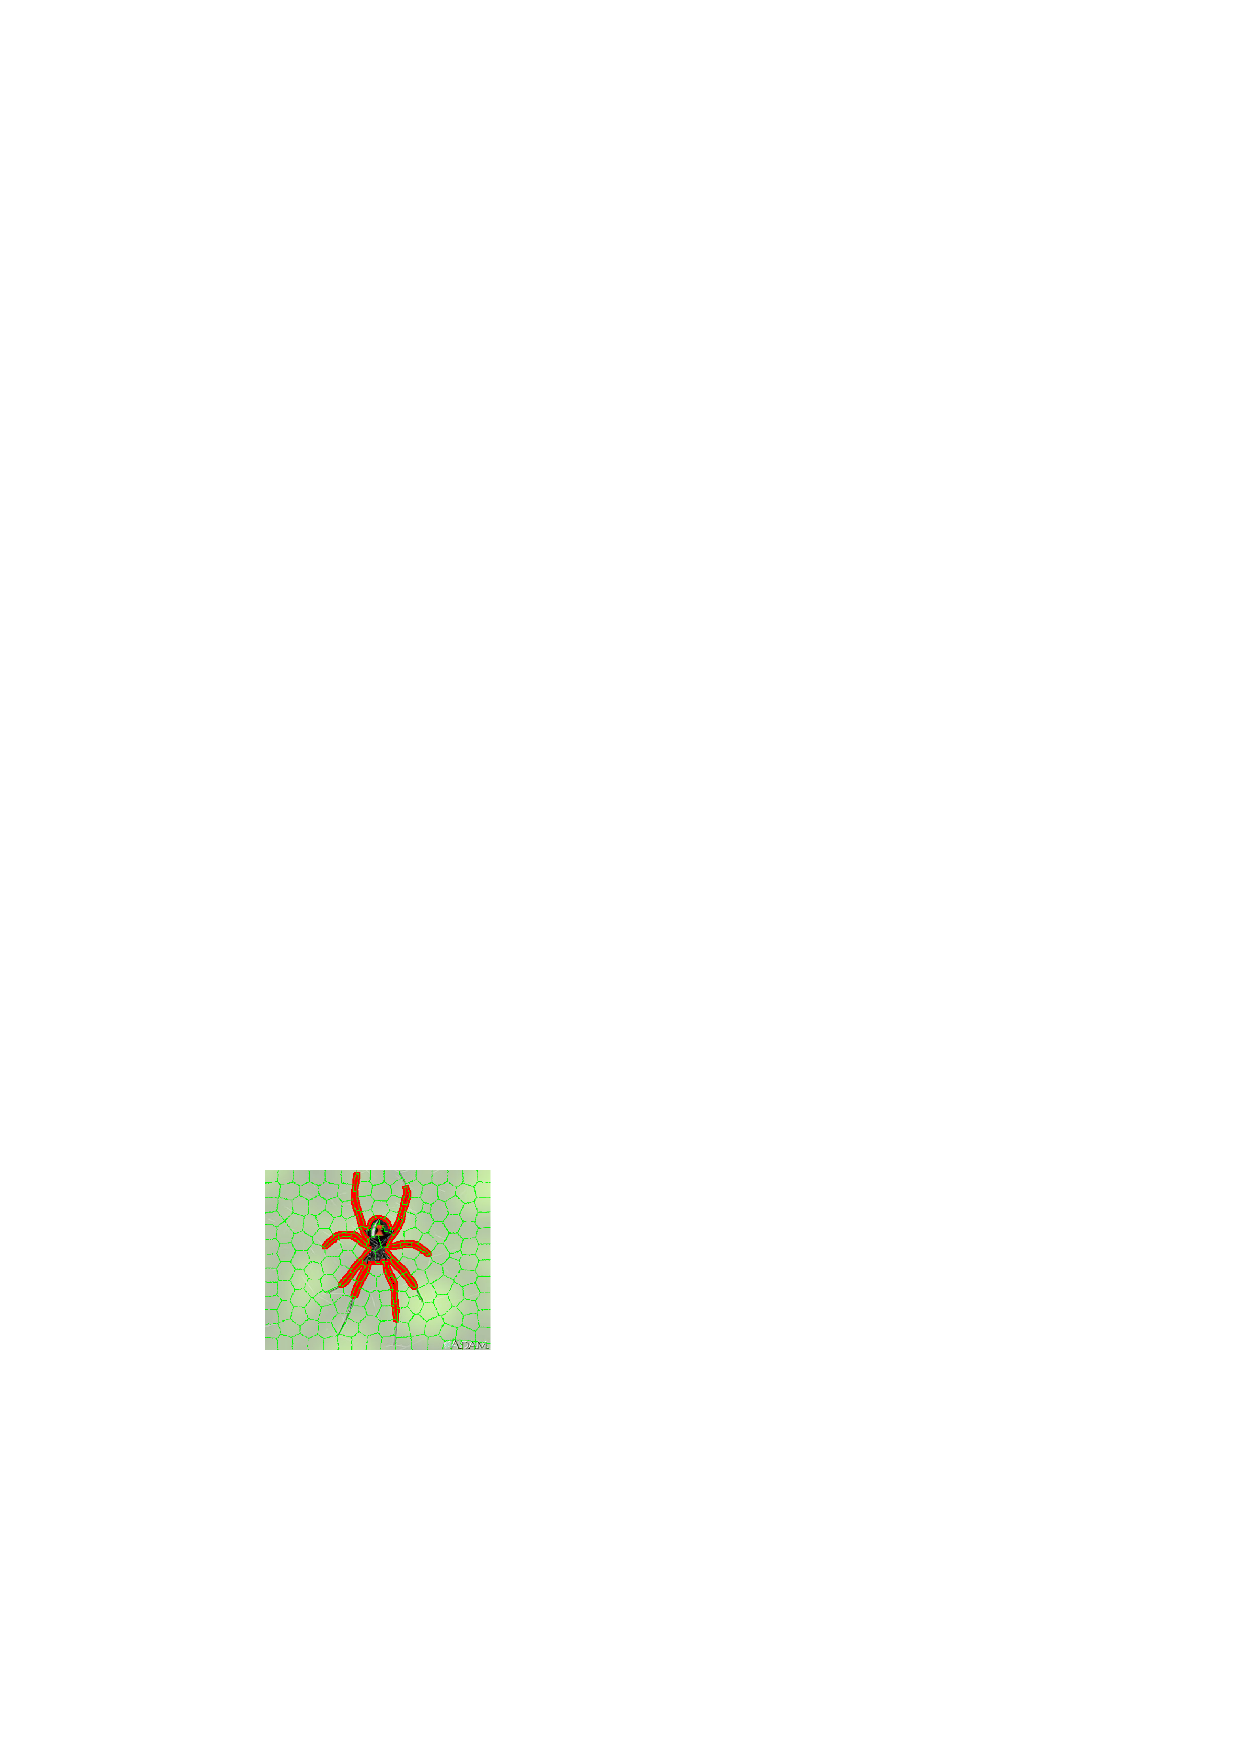
\includegraphics[width=0.15\textwidth]{figs/sp_prob2.pdf}
%% {\footnotesize\textit{c}}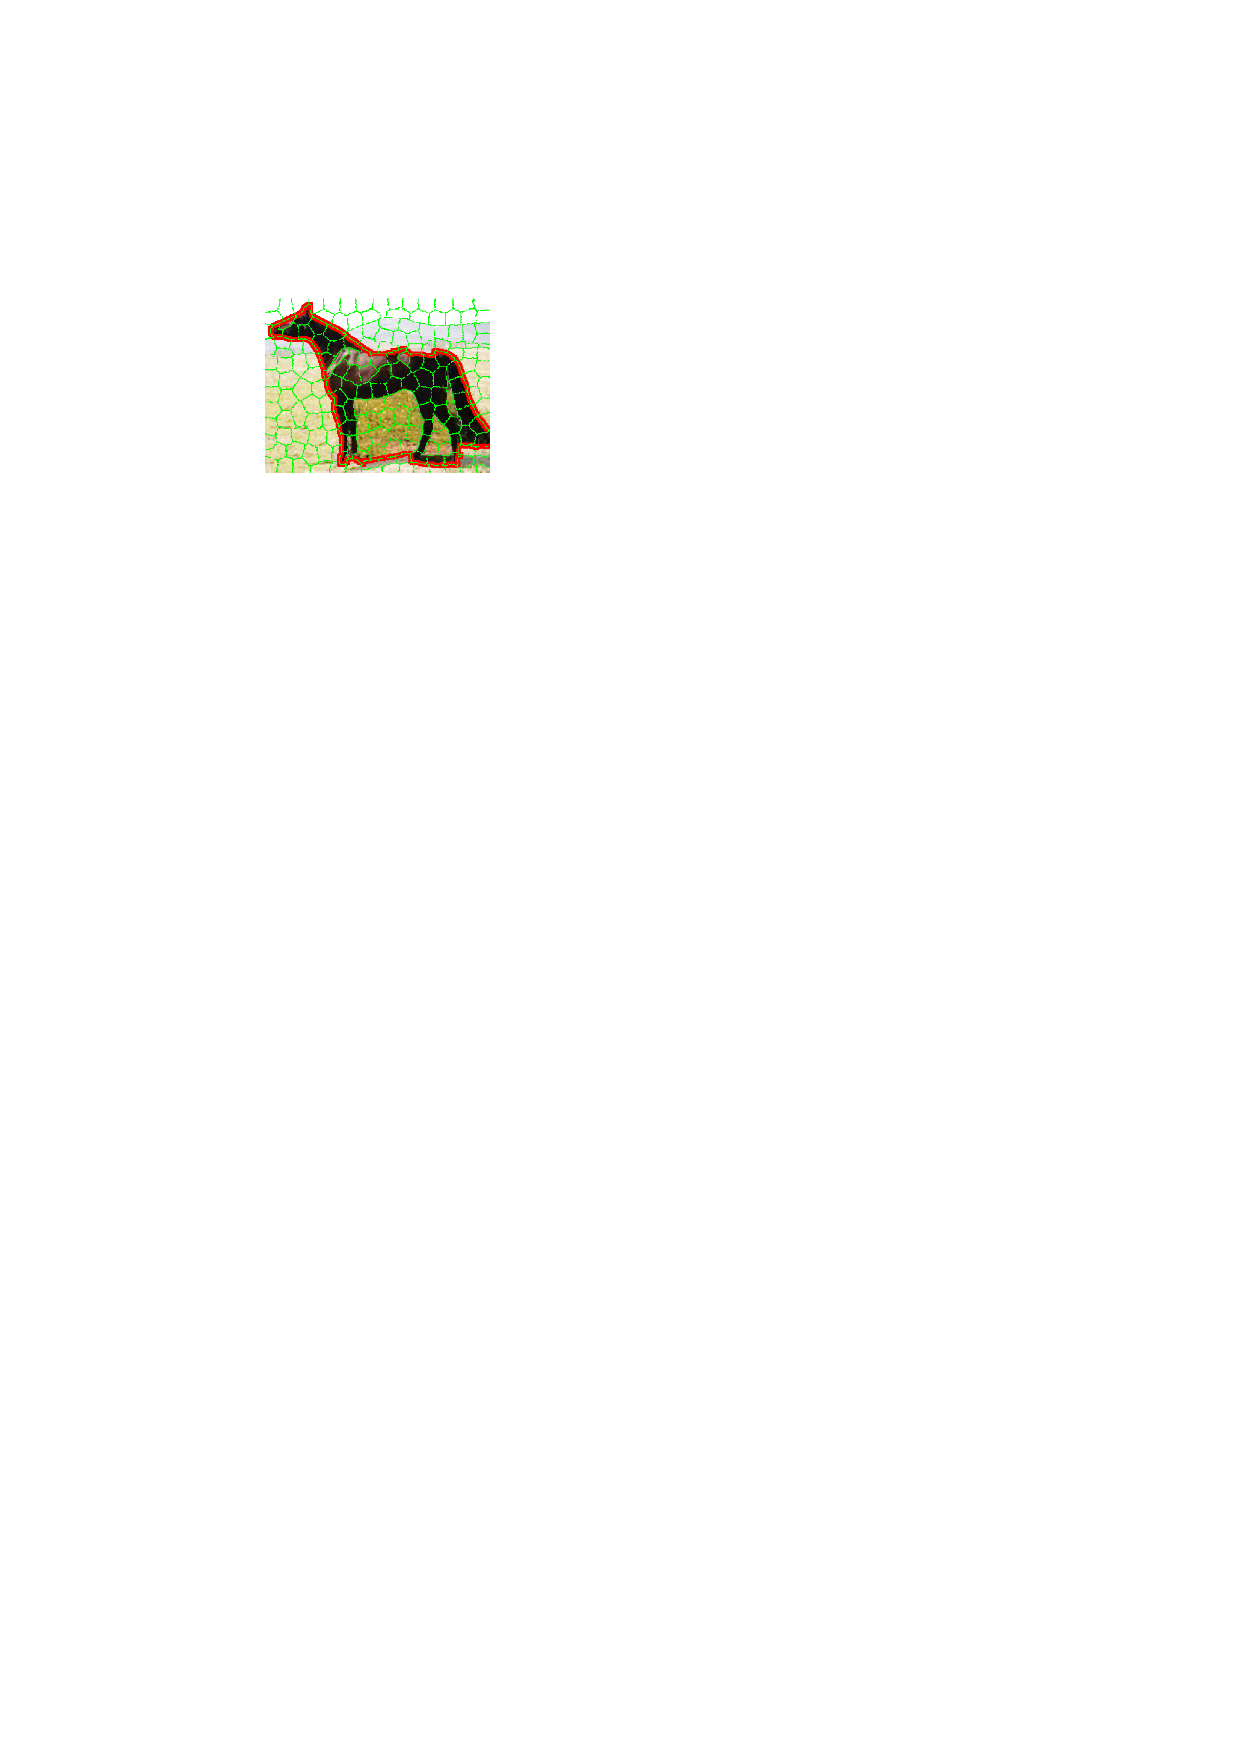
\includegraphics[width=0.15\textwidth]{figs/sp_prob3.pdf}
%% \caption{All images courtesy of~\cite{Levinshtein:etal:IJCV12}. a) A small set of superpixels with the red cycle indicating a possible closed contour to consider. The blue path represents the boundary of a non-closed region. b)c) Examples of successful and erroneous recovery of the object silhouette. }
%% \label{fig:sp_issues}
%% \end{figure}

%% Determining the object boundary utilizing superpixels is a difficult task, irregardless of whether the goal is a closed region or not. The task of recovering the contour amounts to merging the various delimiters, which given a superpixel graph amounts to considering all possible cycles~\cite{Levinshtein:etal:IJCV12}, Figure~\ref{fig:sp_issues}. The red-dashed line in Figure~\ref{fig:sp_issues}\textcolor{red}{a} is one possible cycle out of the many combinations that could possibly exist. We can see successful recovery of the closed contour in Figure~\ref{fig:sp_issues}\textcolor{red}{b}, but the subsequent figure depicts an erroneous recovered boundary despite the superpixels perfectly following the silhouette of the horse. 
%% Representing non-closed regions can be not effectively done by a region based description alone. Superpixels and there consistent boundaries can only represent closed curves, 



 
%% Superpixels are the basic unit of reasoning about object proposals resulting from grouping pixels into region fragments based on regional homogeneity~\cite{Ren:Malik:ICCV03,Ahuja:Todorovic:CVPR08,malisiewicz:bmvc07}.  

%% One main difficulty with the boundaries of  superpixels is that it is not clear which portions are meaningful boundaries and which are simply delimiters of the grouped pixels. These latter contours are more a product of the dynamics of the grouping process than an indicator of underlying structure, \eg, the pink-yellow boundary in Figure~\ref{figure:combinatorial:possibilities}b. The ambiguity created by the presence of these artifactual boundaries among meaningful boundaries limits the use of grouping based on contours.
% \begin{figure}[!h]
% \centerline{
% {\footnotesize\textit{a}}
% \includegraphics[height=0.22\linewidth]{figs/shaded-torus.png}
% {\footnotesize\textit{b}}
% \includegraphics[height=0.22\linewidth]{figs/shaded-torus-segmentation.png}
% {\footnotesize\textit{c}}
% \includegraphics[height=0.22\linewidth]{figs/koenderink-contour-end-1.png}
% {\footnotesize\textit{d}}
% \includegraphics[height=0.22\linewidth]{figs/picasso-hands.png}
% %\includegraphics[height=0.2\linewidth]{figs/Prometheus-Brennan.png}
% %\hspace{-0.1cm}\includegraphics[height=0.2\linewidth]{figs/Prometheus-Brennan-k_12.pdf}
% }
%   \caption{\FigureFont
%   \label{fig:region:issues}
%   (a,b) Region-based grouping produce ``superpixels'' with boundaries composed
%   of both meaningful contours as well as artifactual boundaries resulting
%   from the dynamics of the grouping process which delimits adjacent regions
%   but does not lay claim to boundary-hood. Superpixels cannot represent
% contours that end, (c) from \cite{Koenderink:VanDoorn:Perception82} and
% (d) a Picasso drawing.   }
% %\vspace{-0.35cm}
%\end{figure}

%% Another fundamental difficulty in region-based representation is the inability to represent contours that end, Figure~\ref{figure:combinatorial:possibilities}d, which among others,  significantly limits the detection of gaps, \eg, as present in the bottom and top portions of the inner and outer circles in the shaded torus of Figure~\ref{figure:combinatorial:possibilities}a; It is difficult to work with gaps in the superpixel representation, Figure~\ref{figure:combinatorial:possibilities}b, because end-points of contours are not represented. Despite their limitations, superpixels do have their strengths, namely they exhibit neighborhood structure. For any partitioning ( in the formal sense) of the image, a region adjacency graph defines neighborhood relations between partitions or superpixels. 
  
% \begin{figure}[!h]
% {\footnotesize\textit{a}}
% \includegraphics[height=0.076\linewidth]{figs/good-continuation-1.png}
% {\footnotesize\textit{b}}
% \includegraphics[height=0.076\linewidth]{figs/good-continuation-2.png}
% {\footnotesize\textit{c}}
% \includegraphics[height=0.076\linewidth]{figs/good-continuation-3.png}
% {\footnotesize\textit{d}}
% \includegraphics[height=0.076\linewidth]{figs/good-continuation-4.png}
% {\footnotesize\textit{e}}
% \includegraphics[height=0.076\linewidth]{figs/good-continuation-5.png}
% {\footnotesize\textit{f}}
% \includegraphics[height=0.076\linewidth]{figs/appearance-continuity-1.png}
% {\footnotesize\textit{g}}
% \includegraphics[height=0.076\linewidth]{figs/appearance-continuity-2.png}
%   \caption{\FigureFont
%   \label{fig:contour:continuity}
%   The Gestalt notion of good continuation disambiguates between  the two situations in (a,b), but cannot detect interaction from related contours
% (c-e), which require a notion of figural continuity. (f,g) Appearance continuity is another significant cue. 
%   }
% \end{figure}


%% \begin{figure}[!h]
%% %\vspace{-0.5cm}
%% \centering
%%  % {\footnotesize\textit{(a)}} \includegraphics[width=0.1225\linewidth]{figs/place_holder.pdf}
%% {\footnotesize\textit{a}}
%% \includegraphics[width=0.28\linewidth]{figs/shaded-torus.jpg}
%% {\footnotesize\textit{b}} \includegraphics[width=0.28\linewidth]{figs/shaded-torus-segmentation.jpg}
%% {\footnotesize\textit{c}} \includegraphics[width=0.28\linewidth]{figs/torus_contours_multi_color.pdf}
%% \\
%% %{\footnotesize\textit{(d)}}\includegraphics[width=0.1225\linewidth]{figs/contour-but-not-region.png}
%% %{\footnotesize\textit{(e)}} \includegraphics[width=0.1225\linewidth]{figs/competition-between-two-regions.png}
%% {\footnotesize\textit{d}} \includegraphics[height=0.15\textwidth]{figs/picasso-hands.jpg}
%% \vbox{
%% \hbox{
%% {\footnotesize\textit{e}}
%% \includegraphics[height=0.15\linewidth]{figs/contour-but-not-region.jpg}
%% %\includegraphics[height=0.08\linewidth]{figs/figural-continuity-1.png}
%% {\footnotesize\textit{f}}\includegraphics[height=0.15\linewidth]{figs/figural-continuity-2.jpg}
%% %{\footnotesize\textit{f}}\includegraphics[height=0.06\linewidth]{figs/good-continuation-1.png}
%% }
%% \hbox{
%% {\footnotesize\textit{g)}}\includegraphics[height=0.1\linewidth]{figs/good-continuation-3.jpg}
%% %{\footnotesize\textit{h\includegraphics[height=0.056\linewidth]{figs/good-continuation-2.png}}}
%% {\footnotesize\textit{h}}\includegraphics[height=0.1\linewidth]{figs/good-continuation-4.jpg}
%% }
%% }
%% % \hbox[2cm]{\includegraphics{figs/one-contour-between-two-others.png}
%% % \includegraphics{figs/one-contour-supports-another.png}
%% % \includegraphics{figs/one-gap-supports-another.png}}
%% {\footnotesize\textit{i}}\includegraphics[width=0.23\linewidth]{figs/torus_contours_shocks.pdf}
%% %\textit{k} \hspace{-0.0512cm}
%% %  \includegraphics[width=0.135\linewidth]{figs/place_holder.pdf}
%% %\vspace{-0.2cm}
%%   \caption{ (a,b) The use of superpixels is not appropriate in our
%% approach because (i) artifactual boundaries (say the contour between pink
%% and yellow regions) are not differentiated from actual boundaries,   and
%% (ii) the representation does not identify gap endpoints,  required to identify completion candidates. (c) contour fragment endpoints identify potential gaps. (d) many image contours are not closed (e-f)
%% appearance continuity is a powerful cue in grouping. The spatial interaction
%% among contours prevents some gaps from being considered (g), while supporting
%% others\ (h). (i) The shock graph pairs image contours. }
%%  \label{figure:combinatorial:possibilities}
%% %\vspace{-0.751cm}
%%  \end{figure}

\subsection{Unorganized Set of Curve Fragments}

Reasoning with curve fragments is the second of the classic complementary organization of visual processes into region-based and contour-based. However, the use of curve fragments as a basis for reasoning about images has been largely confined to the perceptual grouping community. Gestalt laws such as good continuation have been formulated in terms of curves. Perhaps this is because reasoning with appearance-similarity requires a notion of regions which is lacking in a contour-based representation, except in the special case of a closed contour. There is some work on using contour fragments for object recognition~\cite{Shotton:Blake:Cipolla:iccv05,Ferrari:Fevrier:Jurie:Schmid:PAMI08, Kumar:Torr:Zisserman:BMVC04}. These papers were unable to generalize to objects whose primary cue is appearance and furthermore were restricted to databases, ETHZ Shape Dataset~\cite{Ferrari:etal:IJCV10} where the objects were depicted exclusively from a side viewpoint, \ie side of a horse, side of a giraffe, where the silhouette contours are most discriminative. However, no object proposal methods use curve fragments as a basis for forming objects or object parts, as we propose here. A key shortcoming preventing this is the observation that, in contrast to superpixels which enjoy a spatial organization via the region-adjacency graph, contour fragments lack a neighborhood structure. The lack of spatial organization renders the practical formulation of Gestalt laws challenging as it is not a-priori clear which pair of curve fragments need to interact. We use the shock graph, which is traditionally a representation of closed curves, to represent the spatial organization of contour fragments, as described next. 

%% Curve fragments provide an alternative set of grouping options when compared to superpixels. One of the major strengths of utilizing curve fragments as compared to regional processes is the reduced set of false positives. In both superpixels and curve fragments we have a similar problem, where by we end up with some real boundaries interspersed with spurious boundaries. While in the case, of superpixels a large portion of the boundaries are due to the artificial dynamics of the region process, in the case of contours this is minimized due to the process being inherently based on image evidence, bottom row of Figure~\ref{fig:sp_probs1}. Along with the reduced set of false positive the contour formation process is generic and leads to a wide variety of curve configurations, Figure~\ref{fig:sp_probs2}\textcolor{red}{f}. 
 %% The classic example of this is the sky problem where by a large homogeneous portion of the image is artificially broken into many pieces as region grouping processes are forced to accumulate region information all across the image. In the case of contours, this situation is minimized as contours are adaptive in the sense as they only fire where image evidence presents itself. 

%% And finally unlike superpixels boundaries, curve fragments represent an ordered set of edgels. \textcolor{red}{To Ben: Why is that contours have less artificial or spurious boundaries compared to superpixels? }

%% Curve fragments provide an alternative set of grouping options when compared to superpixels. One of the major strengths of utilizing curve fragments as compared to regional processes is the reduced set of false positives. In both superpixels and curve fragments we have a similar problem, where by we end up with some real boundaries interspersed with spurious boundaries. While in the case, of superpixels a large portion of the boundaries are due to the artificial dynamics of the region process, in the case of contours this is minimized due to the process being inherently based on image evidence. The classic example of this is the sky problem where by a large homogeneous portion of the image is artificially broken into many pieces as region grouping processes are forced to accumulate region information all across the image. In the case of contours, this situation is minimized as contours are adaptive in the sense as they only fire where image evidence presents itself. And finally unlike superpixels boundaries, curve fragments represent an ordered set of edgels. \textcolor{red}{To Ben: Why is that contours have less artificial or spurious boundaries compared to superpixels? }

%% The use of curve fragments as a basis for further reasoning has been predominantly confined to the perceptual grouping community. As a consequence of this, the majority of gestalt laws such as proximity, good continuation, and symmetry have been formulated in terms of curves as compared to other intermediate-level representations. This represents a strong reason for using contours as these laws which lead to ``good form'' can be effectively be implemented in a computational framework. 

%% Despite the appealing characteristics of curve fragments, they do have their drawbacks. The major and most obvious drawback of contours is that they can not represent regions. Ignoring the special case of a closed contour, a general set of image contours renders reasoning with regional information and generating regional proposals impossible. The other major drawback of working with contours is that a set of contours lacks any organization, \emph{i.e.}, neighborhood structure. Unlike superpixels which have an inherent organization captured by a region-adjacency graph, it is not clear how to define neighbors or the idea of proximity with a set of contours. Even more the elegant formulation of gestalt laws in terms of curves is very difficult to implement in practice due to this lack of spatial organization. This requires a representation where contours and their neighborhood structure are explicitly captured. 

%% In summary, superpixels represent both a region and a boundary. However, as we have shown the vast majority of these superpixel boundaries are artificial. If we exclusively use contours the vast majority are veridical, but it limits our ability to recover and reason with regions. What is needed is a integrated representation that represents the veridical contours, coupled with the regions those contours bound. 



 %% Contours like superpixel's are complete representations when it comes to closed regions but are incomplete representations when it comes to explaining non-closed portions of the image. Revisiting Figure~\ref{fig:mvf_justify}\textcolor{red}{c} we see that the final representation we want is composed of a region bounded by two contours. While a contour representation can represent the red contour, it is unable to represent the blue curve which is a region delimiter and not the output of edge linking. 



%% Many ideas from the gestalt school of thought have been formulated in terms 


%% Curve fragments are often viewed as a precursor to figure-ground segregation and for formulating the Gestalt notion of good continuation,Figure~\ref{fig:mvf_justify}\textcolor{red}{c}, \eg, using elastica \cite{Mumford:Elastic:1994,Williams:Jacobs:NC95} or using the Euler Spiral \cite{Kimia:Euler:Spiral:IJCV03}.






%%  Good continuation is used to disambiguate grouping choices. However, a contour representation cannot take into account the interaction of nearby contours  which may invalidate a completion, Figure~\ref{figure:combinatorial:possibilities}g, or which continuations group the wrong sides of a figure, Figure~\ref{figure:combinatorial:possibilities}e. This representation also cannot strongly encourage the groupings in Figure~\ref{figure:combinatorial:possibilities}h, as it should because it cannot represent ``\textit{figural continuity}'', a very  powerful cue in disambiguating conflicting groupings. Figural continuity requires good continuation of \textit{a pair of contours} that are bound together and that continue together. Finally, another proposed powerful Gestalt cue is   \textit{appearance continuity}, which states that two fragments' grouping depends on the continuity of their appearance, Figure~\ref{figure:combinatorial:possibilities}f. 


\subsection{Shock Graph}
\label{sec:shock_graph}

We propose that the shock graph of contour fragments addresses major shortcomings of each of the two distinct but complementary representations: Superpixels do not explicitly distinguish image curves from region grouping delimiters, and an unorganized set of contours have no notion of regions or neighborhood relationship. First observe that the shock graph can associate a region to each shock graph segment. Given many contour fragments, how can we assign a pixel to a particular contour? The grassfire analogy claims a region for each contour by distance to contours, \ie, a pixel is assigned to the closest contour. In other words, a contour extends its influence as far as the medial axis, see Figure~\ref{fig:ma_motivate}. The Medial Axis therefore “binds” together a pair of contours and identifies the region between them.  In this view the medial axis segment is really just a joint representation of a pair of contours and their intervening region. The shock graph~\cite{Kimia:etal:ECCV:Book,Kimia:etal:Shape:Series:I,Giblin:Kimia:Reconstruction:PAMI03}, a refinement of the Medial Axis, which arises from viewing the medial axis as the locus of singularities (shocks) formed in the course of wave propagation (grass-fire) from a pair of contour elements, Figure~\ref{fig:ma_vs_sg}, and its corresponding computation capture this pairwise relationship between contour elements. Formally, 

\begin{figure}[ht]
\center
a)\raisebox{2.5\height}{\includegraphics[width=0.2\textwidth]{figs/ma_step_1.pdf}}
b)\raisebox{1.8\height}{\includegraphics[width=0.2\textwidth]{figs/ma_step_2.pdf}}
c)\fcolorbox{white}{white}{\includegraphics[width=0.2\textwidth]{figs/ma_step_3.pdf}}
d)\fcolorbox{white}{white}{\includegraphics[width=0.2\textwidth]{figs/ma_step_4.pdf}}
\caption{Motivating the use of the medial axis to capture the regional information of \emph{C1}, depicted in Figures (a) and (b) with another interacting contour \emph{C2} illustrated in (c). (d) The medial axis in the absence of any other information, is the bisector of two regions. } 
\label{fig:ma_motivate}
\end{figure}

\begin{figure}[ht]
\center
\includegraphics[width=0.6\textwidth]{figs/shocks-ma-new.pdf}
\caption{From~\cite{Giblin:Kimia:IJCV03}. The advantage of the shock graph over medial axis is its qualitative description of the boundary: given a medial axis segment any of the six shapes in the top row can occur, while a shock graph segment (a monotonically flowing subsegment of the medial axis) qualitatively represents one type of shape.}
\label{fig:ma_vs_sg}
\end{figure}

\begin{definition}
\label{def:sg}
The shock graph is a directed attributed relational graph, $G=(V,E,A)$, where $V$ is the vertex set of shock nodes, $E$ is the edge set of shock segments, and $A$ is the continuous intrinsic geometry and classification labels, specifically $A$ is the set of unary attributes $a_i$ attached to each vertex $v_i \in V$, namely normal, tangent, time of formation and discrete labels sink, source, or junction. The shock link binary attributes $a_{ij}$ attached to each $e_k=(v_i,v_j) \in E$ consist of length, curvature, and acceleration and discrete labels degenerate, semi-degenerate, or regular. 
\end{definition}





%% We answer this in two parts. First we solve the problem, of how to represent contours while recovering their neighborhood relationship? This relationship is precisely captured by the shock graph! 




There are many approaches to computing the medial axis/shock-graph ranging from topological thinning methods, distance transform methods, curve evolution schemes, and finally computational geometric algorithms.  We adopt the approach of~\cite{Tamrakar:Kimia:Shock}, which is  a hybrid between curve evolution and computational geometric techniques. The main advantage of this scheme over curve-evolution based schemes~\cite{Tek:Wave:Propagation:IJCV03} is that it is designed to work not only with a set of \emph{closed curves} but also with a set of \emph{open (non-closed) curves}. In what follows we highlight the main aspects of computing the shock graph to the extent that it is relevant to this thesis. 



%% \begin{figure*}[ht]
%% \center
%% a)\includegraphics[width=0.3\textwidth]{figs/sc_step1.pdf}
%% b)\includegraphics[width=0.3\textwidth]{figs/sc_step2.pdf}
%% c)\includegraphics[width=0.3\textwidth]{figs/sc_step3.pdf}
%% \caption{A pair of \textcolor{red}{contours} and their bisector. Sub figures b and c show how the introduction of  a new source, invalidates the bisector and determines the valid portion. Also notice the formation of shock nodes at the intersection of bisector curves. } 
%% \label{fig:sc1_steps}
%% \end{figure*}


Formally, the computation of shocks from an unorganized set of curve fragments relies on two key ideas. First, since the shocks arising from points and lines can be analytically computed, the curve fragments can be first approximated by a polyline, namely, a set of line segments that share end points; there are well-known algorithms to achieve this by specifying the expected error~\cite{vxl:webcite}. It is well-known that the bisector of two points is a line, the bisector of two lines is a line, and the bisector of a point and a line is a parabola, Figure~\ref{fig:bisect}. The dynamics of shocks moving on this bisector are less trivial but they can also be calculated analytically. The geometry and dynamics of shocks arising from any isolated pair from a collection of point and line sources is therefore readily available in analytic form and this saves in computation time and provides numerical stability robustness. 

\begin{figure}[ht]
\center
a)\includegraphics[width=0.221\textwidth]{figs/point-point-fixed.pdf}
b)\includegraphics[width=0.4\textwidth]{figs/line-line-fixed.pdf}
c)\includegraphics[width=0.221\textwidth]{figs/point-line-fixed.pdf}

\caption{Analytic computation of shocks from polylines requires shocks from (a) point-point (b) line-line and (c) point-line pairs. Boundary “sources” are shown in red, shocks are shown in green, and the rays connecting boundary sources to respective shocks are shown in dashed lines. These computations assume only a pair of sources with no interaction from other sources so all shocks go off to infinity.  } 
\label{fig:bisect}
\end{figure}

The second key idea is the use of a wave propagation and shock propagation to piece together shocks from multiple pairs of sources in a highly efficient way. Observe that the union of all shock-graph of isolated pairs of sources is a superset of the shock graph of the union of boundary sources, \eg, as in the bisectors shown in grey and green which is a superset of the shock graph shown in green in Figure~\ref{fig:sc2_steps}{(h)}. Consider first the shock points on a bisector of a pair of boundary sources: a shock point is valid if no other waves from sources other than its own sources reach there. In other words, a shock is valid if its time of formation (distance to its sources) is earlier than the time of propagation (distance) to any earlier other source. Since the shock path on any bisector has an initial shock point (shock source), the extent of the valid shock path can be determined by first examining the validity of the shock source itself, the first shock point to form in time. Since a valid shock path can only be potentially terminated at the intersection of two shock paths, these are the only points that need to be examined. This is a key distinction since it discretizes the continuous propagation into a discrete propagation. Thus, the algorithm first computes all shock sources, an $N^2$ computation for $N$ boundary sources, and considers shock paths for the sources in order of time. 

\begin{figure*}[ht]
\center
{\footnotesize\textit{a}}\includegraphics[width=0.235\textwidth]{figs/incremental-voro-02-01.pdf}
{\footnotesize\textit{b}}\includegraphics[width=0.235\textwidth]{figs/incremental-voro-02-02.pdf}
{\footnotesize\textit{c}}\includegraphics[width=0.235\textwidth]{figs/incremental-voro-03-01.pdf}
{\footnotesize\textit{d}}\includegraphics[width=0.235\textwidth]{figs/incremental-voro-03-02.pdf}
{\footnotesize\textit{e}}\includegraphics[width=0.235\textwidth]{figs/incremental-voro-04-01.pdf}
{\footnotesize\textit{f}}\includegraphics[width=0.235\textwidth]{figs/incremental-voro-04-02.pdf}
{\footnotesize\textit{g}}\includegraphics[width=0.235\textwidth]{figs/incremental-voro-05-01.pdf}
{\footnotesize\textit{h}}\includegraphics[width=0.235\textwidth]{figs/incremental-voro-05-02.pdf}

\caption{This figure illustrates the incremental steps of shock computation for a set of \textcolor{red}{red input curves}. At each step infinite length \textcolor{cyan}{cyan bisector curves} between a new boundary element and each of the previous boundary elements are computed. The finite true bisectors after the limiting process are shown in \textcolor{green}{green} with the removed shock branches shown in \textcolor{gray}{gray}. The \textcolor{green}{green shock links} represent the valid portion of bisector curves.} 
\label{fig:sc2_steps}
\end{figure*}


Figure~\ref{fig:sc2_steps} illustrates this process. Consider two fragments, $C_1$ and $C_2$ whose potential shock path is shown in cyan in (a).  For the purpose of illustrating the second key idea, namely using propagation to compute the shock graph, the contour fragments are not restricted to be polylines and can take any form. Also, these are sketches and not accurate in scale. Since there are no other interacting shock paths, the entire shock path is validated and shown in green. Next, suppose that a third contour fragment $C_3$ is added to the pool of curve fragments. The interaction of the new-comer $C_3$ with $C_1$ and $C_2$ generates two potential shock paths shown in cyan in (c). The intersection of these shock paths with existing shock paths create shock junctions, which are the only potential terminators of a shock path. In this particular case there is only one shock junction, with each of the three shock paths flowing into the shock junction. Since the continuation of each shock path has a time exceeding the time of the waves reaching there from another source, all three shock paths are terminated, as shown in (d). In other cases it can happen that two shock branches flow into a junction and one shock branch flows out. In this case the two branches flowing into the junction are terminated in which the shock branch flowing out only begins at the junction as its source. It can also happen that the entire shock path is invalid, say if the two sources on the opposite sides of an image with many sources in between. Consider now $N$ boundary sources. The process of shock computation can be implemented by first computing the shock path for a pair of boundary sources, and then considering a third, a fourth, \etc. , Figure~\ref{fig:sc2_steps}. While this can be done in any order, the most efficient order is one that considers the earliest forming shocks first. 



The practical implementation of these two ideas is realized through the construction and visitation of two time-ordered lists. The first list contains the \emph{candidate} sources that are initially pre-computed and has size $N^2$ and is a superset of all possible source nodes in the shock-graph. The second list is the \emph{active} shock list, the list of shocks under propagation, and is initially empty. The algorithm proceeds by visiting the first element in the \emph{candidate} source list and initializing a pair of child shocks (outgoing flow) where each child has a start time equivalent to the time of formation of the source node and an end time initially at infinity. This initial pair of shocks are inserted into the active elements list, and the source node is removed from the \emph{candidate} list. Each \emph{active} shock is then propagated to the nearest junction on it, thus forming a valid shock link of the shock graph, with a specific start and a specific end-time, and this active shock is now removed from the list. The process is iterated by visiting the next active shock in the list. As the algorithm alternates between visiting the two lists it prioritizes visiting \emph{active} shock elements first over candidate sources. If there are no more active shocks the algorithm will visit the next element in the candidate source list, initialize a new pair of child shocks, and subsequently propagate those active shocks to determine junctions with the existing shocks. This process will terminate when both lists are empty. As candidate sources are visited the algorithm determines which sources are valid or invalid given the current state of the simulation, before initializing a new pair of child shocks. It is formally shown in~\cite{Tamrakar:Kimia:Shock} that the number of discarded candidate sources in the second stage (propagation of shocks) leads to a logarithmic dependency on the number of contours, $N$, resulting in an overall run-time of $N^2log(N)$. Note that during this process, shocks, shock nodes, and shock links are augmented with continuous attributes such as its intrinsic geometry (time of formation, length, curvature, \etc) and also labeled with discrete attributes signifying the \emph{node type}, namely, source, sink, or junction and \emph{link type}, namely, degenerate, semi-degenerate, or degenerate~\cite{Giblin:Kimia:IJCV03}. 









%% and inserts these shocks 

%% each of the $N^2$ candidate sources sequentially, initializes a pair of outgoing (child) shocks from the source node, and subsequently inserts them into the \emph{active} shocks list.   If all active shocks are extinguished then the next 

%% If the wavefronts are quenched for that shock path, then the next candidate source is visited in the time-ordered list. If however, the interaction of the shock path with other sources causes a new shock path to arise then that new element is reinserted into the list with the appropriate time. This process terminates when the list is exhausted. The final result of this second stage is the formation of a set of shock links and shock nodes. The intersection of shock paths or bisector curves creates new shock nodes that are shock junctions.  The formation of shock nodes, limits each shock path to its valid portion of the bisector curve, which we refer to as shock links or shock segments. Shock links capture the relationship between nodes and are directed from newer to older, according to the time of formation of the nodes in the curve evolution process. The set of shock nodes and the connecting shock segments defines a shock graph.






%% \begin{figure*}[ht]
%% \center
%% a)\includegraphics[width=0.22\textwidth]{figs/sc2_step_1.pdf}
%% b)\includegraphics[width=0.22\textwidth]{figs/sc2_step_2.pdf}
%% c)\includegraphics[width=0.22\textwidth]{figs/sc2_step_3.pdf}
%% d)\includegraphics[width=0.22\textwidth]{figs/sc2_step_4.pdf}
%% \caption{A \textcolor{red}{contour} represented by a set of polylines. In a) we see how two adjacent polylines spawn a bisector (dashed \textcolor{green}{- -} line). Subsequent steps b)c) and d) determine the valid portion (solid \textcolor{green}{-} line ) of each bisector curve. Also notice the formation of shock nodes at the intersection of bisector curves. } 
%% \label{fig:sc2_steps}
%% \end{figure*}



%% Formally the shock computation algorithm consists of two stages. Given an input of an unorganized set of contours, approximated by discrete polylines, a set of continuous exact candidate shock paths are analytically computed between all pairs of contour elements (points or lines), Figure~\ref{fig:bisect}. The shock segment lies on the bisector curve of a pair of contour elements augmented with the dynamics of flow corresponding to when the wave-fronts from the two sources come together, the instantaneous velocity of shock points along the curve, and the direction of monotonic flow along the curve.  This refinement of a medial-axis segment to a shock path  The output of the first stage is a set of $N^2$, where $N$ is the number of polyline segments, candidate shock paths of infinite length that are pruned in subsequent stages. A list is maintained of these candidate shock paths that is ordered according to time of formation \ie minimum distance between two boundary elements. 
 
%%  Since the interaction of two sources can be fully invalidated or spatially limited by the presence of other sources, in a second stage, all combinations of shock paths are considered to explore this effect, Figure~\ref{fig:sc2_steps}. 



%% \begin{figure}[ht]
%% \center
%% \includegraphics[width=0.4\textwidth]{figs/shock_computation.pdf}
%% \caption{A set of curves in black and all pairs of bisectors shaded out in gray. The blue curves or shocks represent the valid portions of bisector curves.} 
%% \label{fig:shock_compute}
%% \end{figure}

 


Finally, there are two practical considerations in utilizing the shock computation algorithm of~\cite{Tamrakar:Kimia:Shock}. First, many shock paths extend infinitely beyond the image borders. The addition of a bounding box to the initial set of contour fragments contains the shock paths to a finite, well-defined area. In practice, this bounding box is twice the size of the image, Figure~\ref{fig:shocks_regular}. Second, the approximation of each contour fragment as a polyline generates numerous artifactual shocks at the points of convex discontinuity. The regularization algorithm in~\cite{Tamrakar:Kimia:Shock} recovers the ``true'' shock graph, Figure~\ref{fig:shocks_regular}, \ie, the shock graph of the contour before the polyline approximation, by scoring and removing shock links according to some user-defined threshold. The saliency computed for each shock link measures the amount of deformation of the boundary that is needed for the link to be removed. It is closely related to the ``splice cost'' in~\cite{Sebastian:etal:Shocks:PAMI2004}. In all subsequent figures, unless otherwise noted, the shock computation is depicted with a bounding box twice the size of the image and with $\lambda=1.0$ regularization.  

\begin{figure}[ht]
\centering
{\footnotesize\textit{a}}\includegraphics[width=0.23\textwidth]{figs/calf_nobbox_noreg.pdf}
{\footnotesize\textit{b}}\includegraphics[width=0.23\textwidth]{figs/calf_bbox_reg.pdf}
\caption{a) The set of \textcolor{red}{red contours} and its corresponding shock graph in \textcolor{green}{green}. b) If we augment the contour set with a \textcolor{magenta}{magenta} bounding box and apply regularization ($\lambda=1.0$) we recover the shock graph corresponding to the initial contour, before the polyline approximation. }
\label{fig:shocks_regular}
\end{figure}



%% Since we are possibly dealing with a set of images contours composed of a mix of closed curves and open curves many shock links will not be limited during the formation process as they will extend infinitely beyond the image borders. To deal with this we augment the initial contour set with a bounding box so that during the second stage of shock computation all shock links are limited to a finite length. The other consideration is the issue of regularization. The initial contour set is approximated with a set of discrete polylines, which introduces artificial shock links and nodes. We utilize the regularization process of~\cite{Tamrakar:Kimia:Shock} to recover the ``true'' shock graph, Figure~\ref{fig:shocks_regular}. The previous definition for the shock graph, Equation~\ref{def:sg}, is consistent whether a bounding box and/or regularization is applied. It is important to note, these issues are not particular to the algorithm we are using but are a common problem that all shock computation algorithms face. 


%% A contour map in a) and its corresponding neighborhood structure as captured by the graph proposed in . We can see links are only between endpoints. In the shock graph contours are paired with neighbors by looking at the interacting shock links.



\subsubsection{Shock Graph and spatial organization of Contours}


%% All prior applications of the shock graph~\cite{Sebastian:etal:Shocks:PAMI2004,Ozcanli:Kimia:BMVC07} in the vision community have exclusively focused on this limited view of the shock graph, namely, a discrete sampled version of the shock graph while discarding the input contour set. 

During the shock computation, each shock link is explicitly associated with the pair of contours that spawned that shock segment. This contour information, however, is not retained in the final output of the shock computation algorithm, since the original contours can be fully recovered from the shock graph using Equation. However, the explicit representation of contours and the coupling of shocks and contours is important because the contour neighborhood structure can be explicitly represented by the interacting shock links. The contour topology, knowing which contour neighbors a given contour, is important in contour-based transformations such as gap completion. The role of contour topology in grouping is recognized, \eg, in RatioContour~\cite{Wang:etal:PAMI05}, where the process of extracting salient contours from contour fragments relies on an intermediate representation where neighboring contour fragment are first related through proximity of endpoints, Figure~\ref{fig:curve_ng}. 


%% is not explicitly represented but implicitly captured by the interacting shock links. This stands in contrast to more traditional approaches where a graph defining spatial relationships between contours is computed. Figures~\ref{fig:curve_ng}\textcolor{red}{a,b)} show a random set of curves and the corresponding neighborhood structure as defined in RatioContour~\cite{Wang:etal:PAMI05}. In this graph structure, the nodes of the graph represent the endpoints of contours and the edges in the graph represent all possible valid interactions between pairs of endpoints. 

%% This graph structure and its corresponding computation are pretty common and occurs in a variety of papers related to edge-linking. 




%% We take a more general view where contours are explicitly retained and represented. By explicitly coupling contours with shocks it allows us to provide structure to the unorganized set of contours which is necessary if we are to reason with them. In our representation, 

\begin{figure}[ht]
\centering
{\footnotesize\textit{a)}}\includegraphics[width=0.3\textwidth]{figs/random_curves.pdf}
{\footnotesize\textit{b)}}\includegraphics[width=0.3\textwidth]{figs/random_curves_ng.pdf}
{\footnotesize\textit{c)}}\includegraphics[width=0.3\textwidth]{figs/shock_structure_random_curves.pdf}
\caption{a) A set of image contours taken from~\cite{Wang:etal:PAMI05} and (b) the corresponding graph structure as computed by~\cite{Wang:etal:PAMI05}. (c) The shock graph of the contours in (a) captures the neighborhood structure for this contour map: each shock link establishes a neighborhood relation between two contour fragments. In addition, the type of shock link define endpoint to endpoint neighboring relations. }
\label{fig:curve_ng}
\end{figure}

The shock graph defines a contour topology: each contour interrogates all the shock links it forms for the other contours that formed that shock. In addition, the shock captures both the interactions with interior of a contour or with its endpoints. For example, for the contour $C_7$ in Figure~\ref{fig:curve_ng}\textcolor{red}{(c)}, the shock links $S_1$ and $S_2$ associated with $C_7$ indicate that the endpoints of $C_7$ are the neighbors of $C_2$ and $C_5$. Shock link $S_3$ on the other hand indicates $C_4$ is a neighbor of the contour excluding its endpoints. %% In summary, the shock graph provides a very rich description of neighborhood relationships thats stands in contrast to a more traditional approach where all that can be recovered is the interaction between the endpoints of a set of contours.

%% Compared to existing approaches the spatial organization of contours captured by the shock graph is distinct in two ways: \emph{(i)} the relationship is implicitly captured by the shock links and \emph{(ii)} the shock links capture relationships beyond just endpoints of neighboring contours. Observe how the contour map in Figure~\ref{fig:curve_ng}\textcolor{red}{(a)} spatially organized by ~\cite{Wang:etal:PAMI05} in \textcolor{red}{(b)} is explicitly captured through graph links. In our approach, Figure~\ref{fig:curve_ng}\textcolor{red}{(c)}, the relationship between contours is implicitly captured, \ie, each contour element (point or line) must query its spawned shocks to determine its neighbors. The second difference is the various relationships captured. Consider 

%% we capture neighborhood relationships between the ``full'' contour and not just its endpoints. Observe that in Figure~\ref{fig:curve_ng}\textcolor{red}{c} we have a set of five unorganized contours, $C=\{C_0,...,C_4\}$, with its corresponding shock graph. If we traverse the shock graph counter-clockwise around contour $C_0$ we can observe how each shock link is capturing a neighbor. For example, $S_1$ informs us that $C_1$ is a neighbor on one side, while $S_3$ captures the neighbor $C_4$ on other side. Shock links $S_2$ and $S_4$ capture neighbors $C_2$ and $C_3$ respectively. Not only does the shock graph capture the relative spatial arrangement of $C_0$ neighbors but also it identifies the type of neighborhood relationship. The shock links $S_2$ and $S_4$ are the result of the interaction of the endpoints of $C_0$  with $C_2$ and $C_3$. $C_2$ and $C_3$ represent ``endpoint'' neighbors of $C_0$ while  $C_1$ and $C_4$ represent the ``full'' contour neighbors. The type of neighbor  (endpoint or contour) and spatial arrangement information could be made explicit in a new contour graph, but instead contours simply query their spawned shock links to determine their neighbors. 

%% augment each parametrized contour with a neighborhood table indexed by arc-length, $s$, where $s=0$ and $s=L$, correspond to the neighbors of each contour's endpoints.  


%% In practice, 




%% In our application the shock graph is coupled with the input contour map through way of pointers. In practice we augment each shock edge attribute with pointers to the pair of consistenuent contour elements that spawned it. This subtle technicality means our representation as this point, is not exactly a shock graph as defined by Definition~\ref{def:sg} but rather a new representation which essentially represents contour fragments endowed with neighborhood structure, if you will Contour Fragments++. From this point forward any mention of the shock graph pertains to including the contour structure. 




\subsubsection{Shock Graph Partitions an Image into Regions}
\label{sec:sg_to_regions}


%% The previous section illustrated how the shock graph can be utilized to represent contours and their spatial interaction. While this addresses half the problem, how can we augment the shock graph to recover regions? This represents a major contribution of our work, and to do that we revisit the shock formation process.



A shock point is the quench point of waves from the boundary~\cite{Blum67Transformation}. As such each shock segment is associated with an \emph{influence zone}, namely the propagating waves from the pair of boundaries that quenched at the shock segment, Figure~\ref{fig:influence_zone}. In the grassfire analogy of Blum, the burnt region corresponding to a shock segment is its influence zone. Observe that each non-boundary image pixel uniquely belongs to some influence zone, and the union of all influence zones partitions the image into a set of non-overlapping fragments, Figure~\ref{fig:pipeline}; each with its own coordinate system as described below. 


\begin{figure}[ht]
\centering
a)\includegraphics[width=0.09\textwidth]{figs/two-arc-rays-01.pdf}
\includegraphics[width=0.09\textwidth]{figs/two-arc-rays-03.pdf}
\includegraphics[width=0.09\textwidth]{figs/two-arc-rays-05.pdf}
\includegraphics[width=0.09\textwidth]{figs/two-arc-rays-07.pdf}
\includegraphics[width=0.09\textwidth]{figs/two-arc-rays-final.pdf}
b)\includegraphics[width=0.09\textwidth]{figs/parabola-rays-shocks-01.pdf}
\includegraphics[width=0.09\textwidth]{figs/parabola-rays-shocks-03.pdf}
\includegraphics[width=0.09\textwidth]{figs/parabola-rays-shocks-05.pdf}
\includegraphics[width=0.09\textwidth]{figs/parabola-rays-shocks-08.pdf}
\includegraphics[width=0.09\textwidth]{figs/parabola-rays-shocks-final.pdf}
\caption{The propagating waves in blue traveling from a pair of contours,a), and a single contour,b) quenching at a shock link. Observe how part of the \emph{influence zone} region perimeter is a real \textcolor{red}{contour} while the remaining portion is a \textcolor{blue}{delimiter} of the region only.}
\label{fig:influence_zone}
\end{figure}

\begin{figure*}[!ht]
\centering
{\footnotesize\textit{\textcolor{white}{a)}}}\includegraphics[width=0.228\linewidth]{figs/100075_00.png} 
{\footnotesize\textit{\textcolor{white}{a)}}}\includegraphics[width=0.228\linewidth]{figs/100075_00_cons.pdf} 
{\footnotesize\textit{\textcolor{white}{a)}}}\includegraphics[width=0.228\linewidth]{figs/100075_00_shocks.pdf} 
{\footnotesize\textit{\textcolor{white}{a)}}}\includegraphics[width=0.228\linewidth]{figs/100075_00_atomic_frags.png}
{\footnotesize\textit{\textcolor{white}{a)}}}\includegraphics[width=0.228\linewidth]{figs/134052_00.png}
{\footnotesize\textit{\textcolor{white}{a)}}}\includegraphics[width=0.228\linewidth]{figs/134052_00_cons.pdf}
{\footnotesize\textit{\textcolor{white}{a)}}}\includegraphics[width=0.228\linewidth]{figs/134052_00_shocks.pdf}
{\footnotesize\textit{\textcolor{white}{a)}}}\includegraphics[width=0.228\linewidth]{figs/134052_00_atomic_frags.png}
{\footnotesize\textit{\textcolor{white}{a)}}}\includegraphics[width=0.228\linewidth]{figs/118035_00.png}
{\footnotesize\textit{\textcolor{white}{a)}}}\includegraphics[width=0.228\linewidth]{figs/118035_00_cons.pdf}
{\footnotesize\textit{\textcolor{white}{a)}}}\includegraphics[width=0.228\linewidth]{figs/118035_00_shocks.pdf}
{\footnotesize\textit{\textcolor{white}{a)}}}\includegraphics[width=0.228\linewidth]{figs/118035_00_atomic_frags.png}

%% \includegraphics[width=0.245\linewidth]{figs/153077_00.png} &
%% \includegraphics[width=0.245\linewidth]{figs/153077_00_cons.pdf} &
%% \includegraphics[width=0.245\linewidth]{figs/153077_00_shocks.pdf} &
%% \includegraphics[width=0.245\linewidth]{figs/153077_00_atomic_frags.png}\\
%% \hline
{\footnotesize\textit{\textcolor{white}{a)}}}\includegraphics[width=0.228\linewidth]{figs/173036_00.png} 
{\footnotesize\textit{\textcolor{white}{a)}}}\includegraphics[width=0.228\linewidth]{figs/173036_00_cons.pdf} 
{\footnotesize\textit{\textcolor{white}{a)}}}\includegraphics[width=0.228\linewidth]{figs/173036_00_shocks.pdf} 
{\footnotesize\textit{\textcolor{white}{a)}}}\includegraphics[width=0.228\linewidth]{figs/173036_00_atomic_frags.png}
{\footnotesize\textit{\textcolor{black}{a)}}}\includegraphics[width=0.228\linewidth]{figs/370036_00.png} 
{\footnotesize\textit{\textcolor{black}{b)}}}\includegraphics[width=0.228\linewidth]{figs/370036_00_cons.pdf} 
{\footnotesize\textit{\textcolor{black}{c)}}}\includegraphics[width=0.228\linewidth]{figs/370036_00_shocks.pdf} 
{\footnotesize\textit{\textcolor{black}{d)}}}\includegraphics[width=0.228\linewidth]{figs/370036_00_atomic_frags.png}
%% \includegraphics[width=0.24\linewidth]{figs/000783_con_map.pdf} &
%% \includegraphics[width=0.24\linewidth]{figs/000783_shock_con_map.pdf} &
%% \includegraphics[width=0.24\linewidth]{figs/000783_atomic_fragments_trans.png} &
%% \includegraphics[width=0.24\linewidth]{figs/000783_mvf_fragments_trans.png} \\
%% \hline
%% \includegraphics[width=0.24\linewidth]{figs/001423_con_map.pdf} &
%% \includegraphics[width=0.24\linewidth]{figs/001423_shock_con_map.pdf} &
%% \includegraphics[width=0.24\linewidth]{figs/001423_atomic_fragments_trans.png} &
%% \includegraphics[width=0.24\linewidth]{figs/001423_mvf_fragments_trans.png} \\
%% \hline
%% \includegraphics[width=0.24\linewidth]{figs/001763_con_map.pdf} &
%% \includegraphics[width=0.24\linewidth]{figs/001763_shock_con_map.pdf} &
%% \includegraphics[width=0.24\linewidth]{figs/001763_atomic_fragments_trans.png} &
%% \includegraphics[width=0.24\linewidth]{figs/001763_mvf_fragments_trans.png} \\
%% \hline
%% \includegraphics[width=0.24\linewidth]{figs/002852_con_map.pdf} &
%% \includegraphics[width=0.24\linewidth]{figs/002852_shock_con_map.pdf} &
%% \includegraphics[width=0.24\linewidth]{figs/002852_atomic_fragments_trans.png} &
%% \includegraphics[width=0.24\linewidth]{figs/002852_mvf_fragments_trans.png} \\
%% \hline
%% \includegraphics[width=0.24\linewidth]{figs/001585_con_map.pdf} &
%% \includegraphics[width=0.24\linewidth]{figs/001585_shock_con_map.pdf} &
%% \includegraphics[width=0.24\linewidth]{figs/001585_atomic_fragments_trans.png} &
%% \includegraphics[width=0.24\linewidth]{figs/001585_mvf_fragments_trans.png} \\
%% \hline
%% \includegraphics[width=0.24\linewidth]{figs/001568_con_map.pdf} &
%% \includegraphics[width=0.24\linewidth]{figs/001568_shock_con_map.pdf} &
%% \includegraphics[width=0.24\linewidth]{figs/001568_atomic_fragments_trans.png} &
%% \includegraphics[width=0.24\linewidth]{figs/001568_mvf_fragments_trans.png} \\
%% \hline
%% \includegraphics[width=0.24\linewidth]{figs/003131_con_map.pdf} &
%% \includegraphics[width=0.24\linewidth]{figs/003131_shock_con_map.pdf} &
%% \includegraphics[width=0.24\linewidth]{figs/003131_atomic_fragments_trans.png} &
%% \includegraphics[width=0.24\linewidth]{figs/003131_mvf_fragments_trans.png} \\
%% \hline
\caption{a) The original image and b) its contour map on top of a grayscale version for clarity. c) The shock graph colored in \textcolor{green}{green} (the dynamics are not shown, but are very important) for the associated contour map in \textcolor{red}{red}. d) The \emph{influence zone} associated with each shock segment of the graph partitions the image into regions. We encourage readers to zoom in.}
\label{fig:pipeline}
\end{figure*}

Each shock segment allows for an intrinsic coordinate system to represent its influence zone, one dimension to represent a unique corresponding shock point, and a second dimension to represent distance from the contour~\cite{Giblin:Kimia:Reconstruction:PAMI03}. Specifically, let ${\G}_{k}(s)$ be the shock curve representing a shock segment, where the index $k$ indicates which shock segment, and where $s$ is a length parameter, $s \in [0, L_{k}]$ where $L_{k}$ is the length of the shock link. Let $(\T(s), \N(s))$ represent the tangent and the normal to the shock curve, respectively, where $\T(s)=(\cos(\psi(s),\sin(\psi(s)))$ and $\N(s)=-(\sin(\psi(s)),\cos(\psi(s)))$. Let $v(s)$ be the shock velocity along this curve, and $r(s)$ be the radius of the bi-tangent circle. Let $\varphi$ be the angle between the shock tangent and the ray from the shock to the boundary point; it is shown in~\cite{Giblin:Kimia:Reconstruction:PAMI03} that $v=\frac{1}{cos(\varphi)}$. Then, for each point $p(x,y)$ in the influence zone of the shock segment, there is a unique shock-based coordinate $(s, t), s \in [0, L_{k}], t \in [0,r(s)]$ such that 

\begin{equation}
%p(x,y) = \G_k(s)+t \left( - \frac{1}{v(s)}\T(s)\pm\frac{\sqrt{v(s)^2-1}}{|v(s)|}\N(s) \right).
p(x,y) = \G_k(s) + t(\cos(\varphi)\T(s),\sin(\varphi)\T(s))
\end{equation}

An advantage of this intrinsic coordinate system, is that it allows us to attach appearance descriptors that more closely adhere to the shape of the atomic fragment. The interior of each atomic fragment can be sampled in the natural coordinate frame, $(s,t)$, what in others is referred to as "body-centered coordinates". These two parameters along with the intrinsic fragment orientation, $(\T(s),\N(s))$  define a natural oriented coordinate frame to compute descriptors over. In Figure~\ref{fig:coord_sys_ops}\textcolor{red}{d} we show an example of the novel body centric SIFT descriptors computed in this natural coordinate frame. Notice how the descriptors are aligned with the shape, and thus minimize mixing of foreground and background statistics. Contrast this with Figure~\ref{fig:coord_sys_ops}\textcolor{red}{a} which illustrates the traditional approach of picking a predetermined scale and orientation to compute descriptors. This approach leads to descriptors that do not cover the object of interest (body descriptor) or fall outside the region of interest (descriptor over head),  Figure~\ref{fig:coord_sys_ops}\textcolor{red}{b}. From a practical point of view this allows for a "parameter-free" approach where the orientation and scale do not have to be picked arbitrarily but naturally fall out of the shock graph representation. 

\begin{figure}[ht]
  \centering
  a)\includegraphics[width=0.21\textwidth]{figs/bird_trad_scale.pdf}
  b)\includegraphics[width=0.21\textwidth]{figs/frag_trad_sift.pdf}
  c)\includegraphics[width=0.21\textwidth]{figs/frag_oellipse.pdf}
  d)\includegraphics[width=0.21\textwidth]{figs/frag_sift.pdf}
\caption{(a,b) The traditional computation of SIFT descriptors in object recognition for a fixed orientation and scale. In contrast, the orientation and scale (radius of $r(s)$ determined by the shock graph (c) leads to construction of Body-Centric SIFT~\cite{Lowe:IJCV04} descriptors (d). }
\label{fig:coord_sys_ops}
\end{figure}

\subsection{RECOIN: A New MultiFaceted representation}
\label{sec:representation}

A representation for organizing an image into meaningful candidate object parts must therefore feature: \emph{(i)} an explicit representation of contour fragments to make transforms such as gap completions possible; \emph{(ii)} an explicit representation of regions to allow for grouping of regions based on the appearance of that region; \emph{(iii)} an explicit representation of topology of contours and regions to allow for identifying neighbors with which interactions must take place. Such a representation: is necessarily redundant, and we represent it as three coupled layers, one to represent the set of contour fragments, one to represent the set of regions, and one to represent the shock graph, as described below. Note that our approach is to organize the image by applying a sequence of transforms to the representation, so that a representation at any point in the sequence is indicative of the “state” of the image at some stage of organization 


\noindent\\
{\bf The Contour Fragment Layer: } The contour fragment layer is a collection of contours $\{C_1,C_2,\cdots,C_N\}$. Each contour is represented in some way, for example, as an ordered set of points, or as an ordered set of oriented points (points and tangents). We choose a polyline representation for each contour. The particular form of the representation is not critical. The contour fragment layer must allow for \emph{(i)} addition of new contour fragments, \emph{(ii)} deletion of contour fragments, \emph{(iii)} joining two contour fragments into a single contour fragment, and \emph{(iv)} splitting an existing contour fragment into two contour fragments. A simple yet elegant approach to make this possible is to associate a binary label (``present'',''absent'') to each curve, so that a contour fragment can by deleted by simply changing the label to ``absent''. Second, a new contour fragment can be added by simply augmenting $C_{N+1}$ to the set (say after gap completion) . Third, a curve $C$ can be split, say due to the formation of a $T$ junction into two pieces, say $C_1$ and $C_2$. This is handled by leaving all the information about $C$ intact, but relabeling one portion as $C_1$ and another as $C_2$. This can be done iteratively, \eg, so $C_1$ can be split, \etc, thus creating a hierarchy. Currently, splitting can occur only at the joints in the polyline representation for simplicity. We have found this limiting so in the future a better approach is to allow splits at any point. Finally, two curves $C_1$ and $C_2$ can be joined into a new curve $C$ by simply constructing a hierarchal relationship of a new node $C$ pointing in sequence to $C_1$ and $C_2$. 

The contour fragment layer thus allows for proper modification of the set of curve fragments, represented initially as a set of binary labels, each pointing to a geometric representation, and later as a hierarchal set of labels. This portion of the state space can be compared to another simply by comparing the two sets of hierarchal labels, \eg, if we would like to know whether the result of a sequence of transforms is identical to that of another sequence of transforms. 

\noindent\\
{\bf The Region Layer: } The Region Fragment Layer is a partition of the image $\{R_1,R_2,\cdots,R_N\}$. Each region is a set of pixels represented in some way, \eg, as a common label for all pixels belonging to a region. The Region Fragment Layer must allow for \emph{(i)} grouping two regions into a unified region and \emph{(ii)} split a region into two regions. The representation of regions by labels, similarly to contours, allows for a hierarchal grouping and splitting regions fairly easily. 

\noindent\\
{\bf  The Shock-Graph Layer: } The shock-graph layer is a graph representation of shock nodes and shock links. Every shock link maintains a pointer to the contour fragments gave rise to it. Also, each shock link points to the region that intersects its influence zone. 

The key idea in coupling these three representation is to align the contour, region, and shock representation. Thus, a region should be made up of influence zones, shock links should arise from pairs of contour fragments, \etc The key to this integration is the Medial Visual Fragment.

\begin{definition}
A {\bf Medial Visual Fragment (MVF)} is any connected shock subgraph, together with the corresponding contours, corresponding influence zones, and the image intensities in that area. Since any subgraph of a shock graph is itself made up of smaller subgraphs, the smallest unit simply corresponds to a shock link and two shock nodes in which case the MVF is called an {\bf Atomic Medial Fragment (AMF)}~\footnote{Atomic refers to the fact that the MVF cannot be decomposed any further}. %{\bf Type 1 Medial Visual Fragment} is composed exclusively of {\bf Type 1 AMFs}. {\bf Type 2 Medial Visual Fragment} is composed exclusively of {\bf Type 2 AMFs}
\end{definition}

\begin{figure}[ht]
\center
a)\includegraphics[width=0.2\textwidth]{figs/torus.jpg}
b)\includegraphics[width=0.2\textwidth]{figs/shaded-torus-segmentation.jpg}
c)\includegraphics[width=0.2\textwidth]{figs/torus_contours_shocks.pdf}
d)\includegraphics[width=0.2\textwidth]{figs/torus_mvf.pdf}
\caption{a) A simple image example. b) From~\cite{Tamrakar:Kimia:POCV04} the output of the SWA algorithm~\cite{Sharon:etal:CVPR01}. Notice the regions are bounded by real contour and artificial boundaries. c) We see the shock graph and in (d) we see a collection of Medial Visual Fragments. Notice that each medial visual fragment is bounded by red (real ) contours and blue (virtual) delimiters.}
\label{fig:torus_prob}
\end{figure}

In this new representation, MVFs simultaneously represent contours, region, and image intensity within the fragment. Initially, after computation of the shock graph, the resulting MVFs are Atomic Medial Fragment, but later groupings yield larger medial visual fragments. At a first glance, the MVFs appear like an initial superpixel representation. While this is true and indicative that MVFs have all the capabilities of a region-based/superpixel-based representation, it belies a fundamental distinction. In a region-based representation, the boundaries of a region/superpixels may or may not be actual image contours. Figure~\ref{fig:torus_prob} and previous Figures~\ref{fig:sp_probs1}\textcolor{red}{(g,h)} illustrate that some superpixel boundaries are indeed image contours while others are artifactual in that they are simply a delimiter of a grouping process, with no actual image contour evidence. The ambiguity is resolved in the MVF representation, Figure~\ref{fig:torus_prob}\textcolor{red}{(d)}, because the two types of boundaries are distinguished clearly: \emph{(i)} actual image contours as determined by the initial set of contours resulting from grouping edges, or determined as a result of gap completion as indicated by the red contours in the final MVF region of Figure~\ref{fig:influence_zone}; and, (ii) artificial or virtual contours which are known by our approach to be simply a result of the grouping process which partitions the image into regions ( indicated by blue contours in Figure~\ref{fig:influence_zone}). The ability to distinguish between actual contours and artifactual contours is key to processes such as gap completion where superpixels are unable to explicitly represent end points, or contour clutter removal.


%% MVF regions with these two type of boundaries are indicated in Figure~\ref{fig:torus_prob}\textcolor{red}{(d)}.   




 This distinction leads to two types of MVFs: \emph{(i)} those that are the result of interacting actual contours, which may be silhouettes and thus likely to represent object parts, and \emph{(ii)} those that are the result of interacting contour end-points, and which are likely the spatial glue between object parts. We formally define these two types: 


\begin{definition}
A {\bf Type I Atomic Medial Fragment} is the result of interaction of two image contour fragments excluding their endpoints, i.e., either when an interior contour point from one contour fragment interacts with another contour fragment interior point (possibly including a corner point), Figure~\ref{fig:af_types}(a-b). A {\bf Type I Medial Visual Fragment} is composed exclusively of {\bf Type I AMFs}. 
\end{definition}

\begin{figure}[ht]
  \center
  %\includegraphics[width=0.13\textwidth]{figs/b1.pdf}
  a)\includegraphics[width=0.1\textwidth]{figs/b2.pdf}
  %\includegraphics[width=0.05\textwidth]{figs/b3.pdf}
  b)\includegraphics[width=0.1\textwidth]{figs/a1.pdf}
  c)\includegraphics[width=0.15\textwidth]{figs/af_t3.pdf}
  d)\includegraphics[width=0.15\textwidth]{figs/af_t4.pdf}
  %\includegraphics[width=0.13\textwidth]{figs/a3.pdf}
  \caption{Type 1 Atomic Fragments can be seen in a-b). Figure~\ref{fig:influence_zone} can be classified as Type 1 Atomic Fragments also. Type 2 Atomic Fragments can be seen in in c-d. Notice that since type 2 atomic fragments are composed of endpoints, which have zero arc-length, it leads to very little veridical contour (red) .}
  \label{fig:af_types}
\end{figure}

\begin{definition}
A {\bf Type II Atomic Medial Fragment} is the result of interaction of a contour endpoint with another contour fragment interior or another point (endpoint or corner point), Figure~\ref{fig:af_types}(c-d). A {\bf Type II Medial Visual Fragment} is composed exclusively of {\bf Type II AMFs}. 
\end{definition}

\begin{figure*}[!ht]
\centering
{\footnotesize\textit{\textcolor{white}{a)}}}\includegraphics[width=0.228\linewidth]{figs/3096_00_cons.pdf} 
{\footnotesize\textit{\textcolor{white}{a)}}}\includegraphics[width=0.228\linewidth]{figs/3096_00_labeled_shocks.pdf} 
{\footnotesize\textit{\textcolor{white}{a)}}}\includegraphics[width=0.228\linewidth]{figs/3096_00_type1_atomic_frags.pdf} 
{\footnotesize\textit{\textcolor{white}{a)}}}\includegraphics[width=0.228\linewidth]{figs/3096_00_type2_atomic_frags.pdf} 
{\footnotesize\textit{\textcolor{white}{a)}}}\includegraphics[width=0.228\linewidth]{figs/178054_00_cons.pdf} 
{\footnotesize\textit{\textcolor{white}{a)}}}\includegraphics[width=0.228\linewidth]{figs/178054_00_labeled_shocks.pdf} 
{\footnotesize\textit{\textcolor{white}{a)}}}\includegraphics[width=0.228\linewidth]{figs/178054_00_type1_atomic_frags.pdf} 
{\footnotesize\textit{\textcolor{white}{a)}}}\includegraphics[width=0.228\linewidth]{figs/178054_00_type2_atomic_frags.pdf} 
{\footnotesize\textit{\textcolor{black}{a)}}}\includegraphics[width=0.228\linewidth]{figs/41004_00_cons.pdf} 
{\footnotesize\textit{\textcolor{black}{b)}}}\includegraphics[width=0.228\linewidth]{figs/41004_00_labeled_shocks.pdf} 
{\footnotesize\textit{\textcolor{black}{c)}}}\includegraphics[width=0.228\linewidth]{figs/41004_00_type1_atomic_frags.pdf} 
{\footnotesize\textit{\textcolor{black}{d)}}}\includegraphics[width=0.228\linewidth]{figs/41004_00_type2_atomic_frags.pdf} 
\caption{(a) The image and (b) its shock graph. The links of the shock graph are colored \textcolor{cyan}{cyan} to represent shocks links that have an attached Type I atomic fragment and colored \textcolor{magenta}{magenta} to represent Type II atomic fragments. In subsequent figures we see the attached regions for every shock link.}
\label{fig:atomic_frag_types}
\end{figure*}

Observe that with these definitions, all AMFs are either type I or type II. While the reader may suspect that a third type of MVF is possible as a mix of Type I and Type II AMFs, our processes keep from mixing types, so such addition is not necessary. Figure~\ref{fig:atomic_frag_types} shows the division of AMFs into these two types for several images, with type I shown in the third column and type II in the fourth column. It is evident that the Type I Atomic Medial Fragments which represent the interaction of contours which themselves are purportedly the separators of object boundaries, are the beginning of reasoning about object parts. These Type 1 Atomic Medial Fragments play a critical role in a part-based representation of shape. Observe in Figure~\ref{fig:atomic_frag_zoomin}\textcolor{red}{(a)} how objects within the image are decomposed into semantic notions of parts, \ie, appendages of the star fish, upper and lower portions of legs, and ears of the bear. Our visual reasoning about object proposals begins with these. The type II AMFs, on the other hand, represent the spatial glue between Type I AMFs and represent the layout and interactions. If we examine Type 2 AMFs in the last two columns of Figure~\ref{fig:atomic_frag_zoomin}\textcolor{red}{(b)} we notice that these fragments in general do not correspond to semantic notions of objects or parts. 

\begin{figure*}[!ht]
\centering
%% \includegraphics[width=0.24\linewidth]{figs/113044_00_cropped_cons.pdf} &
%% \includegraphics[width=0.24\linewidth]{figs/113044_00_cropped_type1.pdf} &
%% \includegraphics[width=0.25\linewidth]{figs/42049_00_cropped_cons.pdf} &
%% \includegraphics[width=0.25\linewidth]{figs/42049_00_cropped_type1.pdf} \\
%% \hline
{\footnotesize\textit{\textcolor{white}{a)}}}\includegraphics[height=0.139\linewidth]{figs/12003_00_rc_cons.pdf}
\includegraphics[width=0.137\linewidth]{figs/153077_00_rc_cons.pdf}
\includegraphics[height=0.13\linewidth]{figs/100080_00_rc_cons.pdf}
\includegraphics[height=0.13\linewidth]{figs/157055_00_rc_cons.pdf} 
{\footnotesize\textit{\textcolor{white}{a)}}}\includegraphics[height=0.13\linewidth]{figs/231015_00_rc_cons.pdf} 
\includegraphics[width=0.13\linewidth]{figs/23025_00_rc_cons.pdf} 
{\footnotesize\textit{a)}}\includegraphics[height=0.139\linewidth]{figs/12003_00_rc_before_frags.pdf}
\includegraphics[width=0.139\linewidth]{figs/153077_00_rc_before_frags.pdf}
\includegraphics[height=0.13\linewidth]{figs/100080_00_rc_before_frags.pdf}
\includegraphics[height=0.13\linewidth]{figs/157055_00_rc_before_frags.pdf} 
{\footnotesize\textit{\textcolor{black}{b)}}}\includegraphics[height=0.1385\linewidth]{figs/231015_00_rc_before_frags.pdf} 
\includegraphics[width=0.13\linewidth]{figs/23025_00_rc_before_frags.pdf} 

   
%% \includegraphics[height=0.135\linewidth]{figs/12003_00_rc_before_frags.pdf} 
%% \includegraphics[width=0.145\linewidth]{figs/153077_00_rc_before_frags.pdf}
%% \includegraphics[height=0.14\linewidth]{figs/100080_00_rc_before_frags.pdf} 
%% \includegraphics[height=0.27\linewidth]{figs/157055_00_rc_cons.pdf} 
%% \includegraphics[height=0.27\linewidth]{figs/157055_00_rc_before_frags.pdf}
%% \includegraphics[height=0.21\linewidth]{figs/231015_00_rc_cons.pdf} 
%% \includegraphics[height=0.21\linewidth]{figs/231015_00_rc_before_frags.pdf} 
%% \includegraphics[width=0.21\linewidth]{figs/23025_00_rc_cons.pdf} 
%% \includegraphics[width=0.21\linewidth]{figs/23025_00_rc_before_frags.pdf}

%% \includegraphics[width=0.24\linewidth]{figs/ex3_af_to_mvf_s1.pdf} &
%% \includegraphics[width=0.24\linewidth]{figs/ex3_af_to_mvf_s2.pdf} &
%% \includegraphics[width=0.24\linewidth]{figs/ex3_af_to_mvf_s3.pdf} \\
%% \hline
%% \includegraphics[width=0.24\linewidth]{figs/ex2_af_to_mvf_s1.pdf} &
%% \includegraphics[width=0.24\linewidth]{figs/ex2_af_to_mvf_s2.pdf} &
%% \includegraphics[width=0.24\linewidth]{figs/ex2_af_to_mvf_s3.pdf} \\
%% \hline
%% \includegraphics[width=0.24\linewidth]{figs/ex4_af_to_mvf_s1.pdf} &
%% \includegraphics[width=0.24\linewidth]{figs/ex4_af_to_mvf_s2.pdf} &
%% \includegraphics[width=0.24\linewidth]{figs/ex4_af_to_mvf_s3.pdf} \\
%% \hline
%% \includegraphics[width=0.24\linewidth]{figs/ex1_af_to_mvf_s1.pdf} &
%% \includegraphics[width=0.24\linewidth]{figs/ex1_af_to_mvf_s2.pdf} &
%% \includegraphics[width=0.24\linewidth]{figs/ex1_af_to_mvf_s3.pdf} \\
%% \hline


\caption{(a) The top shows zoomed in portions of images and their contour map while in the bottom row Type I atomic fragments are highlighted. Notice for many of the examples these Type 1 MVFs correspond to semantic notions of parts. (b) The top row again shows zoomed in portions of images and their contour map. The bottom row shows Type II atomic fragments which do not offer a semantic interpretation. }
\label{fig:atomic_frag_zoomin}
\end{figure*}

%An image is partitioned into a set of influence zones by the shock graph. The result of grouping these produces a set of regions $\{R_1,R_2,\cdots,R_N\}$ These regions are defined as part of a more complex representation, which includes region, but also contours and their spatial organization. 




While the major difference between superpixels and MVFs is the ability to represent contours another important difference is the neighborhood structure between our Medial Visual Fragments compared to superpixels. Each shock link corresponds to a region and shock nodes capture lateral neighborhood relationships which contour fragments represent transversal neighborhood relations.  The mapping is reversed in a region adjacency graph where each \emph{node} corresponds to a region and each \emph{edge} captures the neighbors. If we take the dual of the shock graph we end up with a RAG representation, Figure~\ref{fig:ng}.  The shock graph neighborhood structure is a drastically reduced subset of the edges of the RAG of AMFs. One disadvantage of the shock graph neighborhood structure is that the graph can become disconnected if the initial contour map, is composed of closed curves. For example, the shock graph representing the wheels of a car tend to become disconnected from the shock graph capturing the body of a car.

\begin{figure}[ht]
\centering
a)\includegraphics[width=0.225\textwidth]{figs/24004_00.png}
b)\includegraphics[width=0.225\textwidth]{figs/24004_afs.pdf}
c)\includegraphics[width=0.225\textwidth]{figs/24004_sg.pdf}
d)\includegraphics[width=0.225\textwidth]{figs/24004_rag.pdf}
\caption{The original image in a) and the corresponding atomic fragments shown in b). Figure c) shows the neighborhood structure versus the neighborhood structure utilizing a region adjacency graph (8 neighborhood connectivity) in d). }
\label{fig:ng}
\end{figure}

%
%
%Image contour fragments, the shock graph that spatially relates and organizes these contour fragments, and the partitioning of the image into the influence zone of individual shock segments can be consolidated into an integrated representation, Figure~\ref{fig:layers}. 

We refer to this ``layered'' representation as RECOIN, Definition~\ref{def:recoin}, as it ties together \{RE\}gions, \{CO\}ntours, and image \{IN\}tensities associated with each region.

\begin{definition}
The {\bf RECOIN} representation is composed of a set of contours $C=\{C_1,C_2,...,C_N\}$, a shock graph , $G=(V,E,A)$, and a set of regions $R=\{R_1,R_2,...,R_M\}$ and their associated image intensities. 
\label{def:recoin}  
\end{definition}

The simultaneous and coupled nature of RECOIN is what makes our representation work. Even if superpixels and unorganized set of contours were perfect, there is no clear way to reason about them simultaneously. We would have to reason with each separately and somehow merge their conflicting evidence in an efficient manner. Because the RECOIN representation begins with atomic medial fragments where all three representations are consistent and synchronized and because in all transformations all three representations remain consistent, the coupled representation remains valid at all times. This powerful representation which allows for a range of transformation due to the explicit simultaneous representation of contours and regions, and their spatial layout, comes at the price of having to maintain a redundant representation. In our implementation we generate the region-based layer fresh in each transformation. In future implementations we plan to have a direct representation, Figure~\ref{fig:layers}.  


%\begin{definition}
%A {\bf Medial Visual Fragment (MVF)} is any connected shock subgraph, together with the corresponding contours, corresponding influence zones, and the image intensities in that area. Since any subgraph of a shock graph is itself made up of smaller subgraphs, the smallest unit simply corresponds to a shock link and two shock nodes in which case the MVF is called an {\bf Atomic Medial Fragment (AMF)}~\footnote{Atomic refers to the fact that the MVF cannot be decomposed any further}. {\bf Type 1 Medial Visual Fragment} is composed exclusively of {\bf Type 1 AMFs}. {\bf Type 2 Medial Visual Fragment} is composed exclusively of {\bf Type 2 AMFs}
%\end{definition}

\begin{figure}[ht]
\centering
\raisebox{-0.5\height}{{\footnotesize\textit{a)}}\includegraphics[width=0.35\textwidth]{figs/layers.png}}
\raisebox{-0.8\height}{{\footnotesize\textit{b)}}}
  \begin{tabular}{p{1.4cm}|p{1.1cm}|p{1.1cm}|p{0.9cm}|p{0.9cm}|}
    \cline{2-5}
    & Contour & Super Pixels & Shock Graph & Ours \\
    \hline
    \multicolumn{1}{|p{2cm}|}{Represent Regions } & Only if Closed & Yes & Yes (Implicit) & Yes\\
    \hline
    \multicolumn{1}{|p{2cm}|}{Represent Contours } & Yes & No & Yes & Yes\\
    \hline
    \multicolumn{1}{|p{2cm}|}{Represent Neighboring Contours } & No & No & Yes & Yes\\
    \hline
    \multicolumn{1}{|p{2cm}|}{Represent Neighboring Regions } & No & Yes (RAG)  & No & Yes\\
    \hline
  \end{tabular}
\caption{a) Our RECOIN representation can be viewed as a set of layers. (b) The strengths/weaknesses of the various representations. Notice how the RECOIN overcomes the deficiencies of all the other approaches, while retaining their strengths.}
\label{fig:layers}
\end{figure}
%In this new representation, MVFs simultaneously represent contours, region, and image intensity within the fragment. Initially, after computation of the shock graph, the resulting MVFs are Atomic Medial Fragment, but later groupings yield larger medial visual fragments. At a first glance, the AMF or MVFs appear like an initial superpixel representation or superpixel representation after some initial grouping, respectively. While this is true and indicative that MVFs have all the capabilities of a region-based/superpixel-based representation, it belies a fundamental distinction. In a region-based representation, the boundaries of a region/superpixels may or may not be actual image contours. Figure~\ref{fig:torus_prob} and previous Figures~\ref{fig:sp_probs1}\textcolor{red}{(g,h)} illustrate that some superpixel boundaries are indeed image contours while others are artifactual in that they are simply a delimiter of a grouping process, with no actual image contour evidence. In contrast, in the MVF representation, Figure~\ref{fig:torus_prob}\textcolor{red}{(d)}, regions have two types of boundaries: \emph{(i)} actual image contours as determined by the initial set of contours resulting from grouping edges, or determined as a result of gap completion as indicated by the red contours in the final MVF region of Figure~\ref{fig:influence_zone}; and, (ii) virtual contours which are known by our approach to be simply a result of the grouping process which partitions the image into regions ( indicated by blue contours in Figure~\ref{fig:influence_zone}). 
%
%
%%% MVF regions with these two type of boundaries are indicated in Figure~\ref{fig:torus_prob}\textcolor{red}{(d)}.   
%
%
%\begin{figure}[ht]
%\center
%a)\includegraphics[width=0.2\textwidth]{figs/torus.jpg}
%b)\includegraphics[width=0.2\textwidth]{figs/shaded-torus-segmentation.jpg}
%c)\includegraphics[width=0.2\textwidth]{figs/torus_contours_shocks.pdf}
%d)\includegraphics[width=0.2\textwidth]{figs/torus_mvf.pdf}
%\caption{a) A simple image example. b) From~\cite{Tamrakar:Kimia:POCV04} the output of the SWA algorithm []. Notice the regions are bounded by real contour and artificial boundaries. c) We see the shock graph and in (d) we see a collection of Medial Visual Fragments. Notice that each medial visual fragment is bounded by red (real ) contours and blue (virtual) delimiters.}
%\label{fig:torus_prob}
%\end{figure}



%% \noindent\\
%% {\bf Intrinsic Coordinate System: } 






%% The notion that shock links pair contour fragments and at the same time represent regions between contour fragments naturally lends to a new multi-faceted representation that effectively addresses the issues and drawbacks discussed earlier with superpixel-based and contour-based approaches. In this new representation, contours and regions are simultaneously represented though a coupled representation of two layers, a layer of contour fragments and a layer of superpixel-like image regions, mediated and coupled by the shock graph layer, Figure~\ref{fig:layers}(a).  This ``layered'' representation allows us to effectively reason about just contours, just regions, or both simultaneously.







%% %% \noindent


%% %% If we consider the portion of the image in the influence zone of a shock link we can associate all pixels with that shock link. Every pixel uniquely belongs to some influence zone, and the union of all influence zones associated with each shock link partitions the image into a set of non-overlapping fragments. If we consider not only the region of the image defined by the influence zone, but also the contours and shock link associated with that portion of the image, we arrive at an integrated representation, which we refer to as \emph{medial visual fragments}, Figure~\ref{fig:pipeline}.


%% %% The shock graph representation by itself does not explicitly hold any regional information, but rather each shock link is implicitly associated with an 




%% %% \begin{figure*}[!ht]
%% %% \centering
%% %% \setlength{\tabcolsep}{1pt}
%% %% \begin{tabular}{|c|c|c|c|}
%% %% \hline
%% %% Image/Contours & Type 1 Atomic Fragments & Image/Contours & Type 1 Atomic Fragments\\
%% %% \hline
%% %% %% \includegraphics[width=0.24\linewidth]{figs/113044_00_cropped_cons.pdf} &
%% %% %% \includegraphics[width=0.24\linewidth]{figs/113044_00_cropped_type1.pdf} &
%% %% %% \includegraphics[width=0.25\linewidth]{figs/42049_00_cropped_cons.pdf} &
%% %% %% \includegraphics[width=0.25\linewidth]{figs/42049_00_cropped_type1.pdf} \\
%% %% %% \hline
%% %% \includegraphics[height=0.22\linewidth]{figs/12003_00_rc_cons.pdf} &
%% %% \includegraphics[height=0.22\linewidth]{figs/12003_00_rc_before_frags.pdf} &
%% %% \includegraphics[width=0.23\linewidth]{figs/153077_00_rc_cons.pdf} &
%% %% \includegraphics[width=0.23\linewidth]{figs/153077_00_rc_before_frags.pdf} \\
%% %% \hline
%% %% \includegraphics[height=0.21\linewidth]{figs/100080_00_rc_cons.pdf} &
%% %% \includegraphics[height=0.21\linewidth]{figs/100080_00_rc_before_frags.pdf} &
%% %% \includegraphics[height=0.22\linewidth]{figs/157055_00_rc_cons.pdf} &
%% %% \includegraphics[height=0.22\linewidth]{figs/157055_00_rc_before_frags.pdf} \\
%% %% \hline
%% %% Image/Contours & Type 2 Atomic Fragments & Image/Contours & Type 2 Atomic Fragments\\
%% %% \hline
%% %% \includegraphics[height=0.21\linewidth]{figs/231015_00_rc_cons.pdf} &
%% %% \includegraphics[height=0.21\linewidth]{figs/231015_00_rc_before_frags.pdf} &
%% %% \includegraphics[width=0.21\linewidth]{figs/23025_00_rc_cons.pdf} &
%% %% \includegraphics[width=0.21\linewidth]{figs/23025_00_rc_before_frags.pdf} \\
%% %% \hline

%% %% %% \includegraphics[width=0.24\linewidth]{figs/ex3_af_to_mvf_s1.pdf} &
%% %% %% \includegraphics[width=0.24\linewidth]{figs/ex3_af_to_mvf_s2.pdf} &
%% %% %% \includegraphics[width=0.24\linewidth]{figs/ex3_af_to_mvf_s3.pdf} \\
%% %% %% \hline
%% %% %% \includegraphics[width=0.24\linewidth]{figs/ex2_af_to_mvf_s1.pdf} &
%% %% %% \includegraphics[width=0.24\linewidth]{figs/ex2_af_to_mvf_s2.pdf} &
%% %% %% \includegraphics[width=0.24\linewidth]{figs/ex2_af_to_mvf_s3.pdf} \\
%% %% %% \hline
%% %% %% \includegraphics[width=0.24\linewidth]{figs/ex4_af_to_mvf_s1.pdf} &
%% %% %% \includegraphics[width=0.24\linewidth]{figs/ex4_af_to_mvf_s2.pdf} &
%% %% %% \includegraphics[width=0.24\linewidth]{figs/ex4_af_to_mvf_s3.pdf} \\
%% %% %% \hline
%% %% %% \includegraphics[width=0.24\linewidth]{figs/ex1_af_to_mvf_s1.pdf} &
%% %% %% \includegraphics[width=0.24\linewidth]{figs/ex1_af_to_mvf_s2.pdf} &
%% %% %% \includegraphics[width=0.24\linewidth]{figs/ex1_af_to_mvf_s3.pdf} \\
%% %% %% \hline

%% %% \end{tabular}
%% %% \caption{Here we see a more zoomed in view of medial visual fragments. In these local pictures we can see that many Type 1 atomic fragments capture semantic notions of parts. In the bottom we see type 2 atomic fragments, that are indicated by the diamond structure, which represents endpoints of contours. } 
%% %% \label{fig:atomic_frag_zoomin}
%% %% \end{figure*}



%% %% \begin{proposition}
%% %% The shock graph, Definition~\ref{def:sg}, of an image $I$ with an associated contour map induces a full partition of $I$ into a set of non-overlapping regions where each edge of the shock graph is a one to one mapping with a region.   
%% %% \end{proposition}

%%  %% Each \emph{medial visual fragment} is analogous to superpixels and form the basic unit of perceptual reasoning. While they share common characteristics to superpixels, we outline major differences between our fragments and superpixels. 

%% We refer to each region of our representation, Figure~\ref{fig:pipeline}\textcolor{red}{(d)}, as a \emph{medial visual fragment}. 




%% %% \begin{figure}[ht]
%% %% \center
%% %% \includegraphics[width=0.3\textwidth]{figs/atomic_fragment.pdf}
%% %% \caption{An atomic fragments is the “influence zone” of each shock segment. Each point $P_i$ in this region has a closest contour point $P^+$ which in turn maps to a shock point $P$. Observe how part of the shock fragment perimeter is a real \textcolor{red}{contour} while the remaining portion is a \textcolor{blue}{delimiter} of the region only.} 
%% %% \label{fig:atomic_fragment}
%% %% \end{figure}


 
%% %% It should be noted that the shock graph induces a full partition of the image into a set of planar regions, where each edge of the graph corresponds to an atomic fragment. In this sense, the regional partition without the remaining shock geometry, flow, label and the associated contour representation is a superpixel representation of the image. 

%% %% We highlight some properties of atomic fragments that make them amenable to further reasoning

%% %It is quite straightforward, therefore, to associate an appearance descriptor with each AMF/MVF to be used for object recognition or further grouping.


%% %% Observe that Atomic Medial Fragments are a complete partition of the image, Figure~\ref{fig:pipeline}, and in that sense AMFs can act like superpixels. While our fragments share many common characteristics with superpixels there are many distinct differences which we outline.  
%% \\
%% %% Also, observe that in, Figure~\ref{fig:pipeline} Column 4, many of the atomic Medial Fragments correspond to semantic notions of parts, but this discussion is beyond the scope of this paper.


%% %% While our fragments share many common characteristics with superpixels there are many distinct differences.
%% %%\noindent
%% %% {\bf Representation of Contours: } The most important difference between medial visual fragments and superpixels is that each MVF is bounded by a set of contours. If we revisit, Figure~\ref{fig:influence_zone}, we notice that the shape of the \emph{influence zone} is determined by a set (one or more) of \textcolor{red}{real} contours and a pair of orthogonal rays emanating from the shock nodes. These \textcolor{blue}{\emph{virtual}} contours coupled with the set of \textcolor{red}{\emph{real}} contours defines a closed boundary for each MVF. \emph{Real} contours do not necessarily mean that they are veridical image contours but rather they are the result of contour formation rather than artificial boundaries between medial visual fragments. If we take an Euler tour of the subgraph defining each MVF we can recover this composite contour boundary composed of real and virtual pieces. By explicitly representing contours each MVF is able to reason with the endpoints associated with these \textcolor{red}{\emph{real}} contours while avoiding the \textcolor{blue}{\emph{virtual}} contours. The ability to represents contours and endpoints is in stark contrast to superpixels where all that can be recovered is the orderless closed perimeter of each region. 



%% %% If we revisit, Figure~\ref{fig:influence_zone} each influence zone is formed by a pair of contour boundaries or a single contour that propagated the waves, but also the shape of the region is bounded by the pair of the orthogonal rays emanating from the shock nodes.  
%% %% \noindent

%% %% \begin{figure}[ht]
%% %% \center
%% %% \includegraphics[width=0.2\textwidth]{figs/atomic_fragment.pdf}
%% %% \caption{An synthetic example of a medial visual fragment. The shaded green region represents the \emph{influence zone}. Observe how part of the shock fragment perimeter is a real \textcolor{red}{contour} while the remaining portion is a \textcolor{blue}{delimiter} of the region only.} 
%% %% \label{fig:atomic_fragment}
%% %% \end{figure}

%% %{\bf Virtual/Real Contours:} Given that each \emph{medial visual fragment}



%%  %% is associated with a single shock link it also inherits the pair of contour boundaries that spawned the shock segment. This pair of contour boundaries can either be two distinct contours, a single contour that interacts with itself, a pair of contour points, or a point and a contour, Figure~\ref{fig:af_types}. Another set of contours is the pair of orthogonal rays emanating from the two shock nodes. 



%% %% If we assume that all objects in an image are composed of some image boundaries, then the ability to represent contours allows us to determine which MVF's are precursor's to full objects or parts and those that are not. Intuitively we would like to reason only with those MVF's where the closed boundary of the subgraph is composed of more \emph{real} contour pieces, versus \emph{virtual}, Equation~\ref{eq:cr}

%% %% \begin{equation}
%% %% Contour_{Ratio}=\frac{\int_0^Lrealds}{\int_0^Lrealds+\int_0^Lvirtualds}
%% %% \label{eq:cr}
%% %% \end{equation}

%% %% \noindent
%% %% Medial Visual Fragments that maximize Equation~\ref{eq:cr} are likely to represent objects and as such we should reason exclusively with those fragments while avoiding MVF's where the \emph{$Contour_{ratio}$} is minimum. The ability to differentiate real and virtual contours allows us a precise way to determine those medial visual fragments likely to represent objects. The key to this distinction is that the interior portion of a contour is seen as separating two objects while the end point of a contour captures the region not yet explained by objects. We can catalog medial visual fragments into object and non-object types by looking at its constituent atomic medial fragments. 






%% %% Given that each shock link is the result of an interaction of a pair of contour elements, we can 

%% %% medial visual fragments according to how much of its boundary is composed of \emph{real} pieces. 


%% %% Intuitively we would like to reason only with those \emph{atomic medial fragments} that are composed of mostly \emph{real} boundary versus virtual. The shock link associated with atomic fragments gives us a practical way to identify those type of atomic fragments. As discussed earlier ...\textcolor{red}{to ben: needs to be fixed} each shock link is the result of the interaction of a pair of lines, or a pair of points, or a line and point. Any atomic fragment that...

%% %% By comparing the arc-length of real contours to the total arc-length of the closed boundary, Equation it gives us a sense of how meaningful each atomic fragment is. 


%% %% Intuitively atomic fragments with 

%% %% \begin{definition}
%% %% Type 1 Atomic Fragments ...
%% %% \end{definition}

%% %% \begin{definition}
%% %% Type 2 Atomic Fragments ...
%% %% \end{definition}



%% %% We shall see in the next section, that the perceptual grouping operations on the image can be cast as manipulation and grouping of MVFs with the goal that this should lead to more regularized MVFs, i.e., ones which increasingly resemble objects and their parts. Thus, MVFs are the basic representation for visual reasoning in our framework. 







%% We have articulated many characteristics of medial visual fragments that make appealing as a fundamental unit for visual reasoning. We show in the subsequent sections, that the perceptual grouping operations on the image can be cast as manipulation and grouping of MVFs with the goal that this should lead to more regularized MVFs, \ie, ones which increasingly resemble objects and their parts. 

%% %% \subsubsection{Grouping Atomic Fragments}
%% %% \label{sec:grouping}

%% %% \textcolor{red}{To Ben: In our outline we agreed to move how we go from atomic fragments to MVF as a transform, the insertion of region transforms. I am not sure where to draw the line, between what we say here and what we leave to the future section. Even more, I described this process, in a totally different but equivalent way in Section~\ref{sec:rg_transform}. Pleae help! }

%% %% We have shown how regional information is appended to the shock graph in the way of atomic fragments, however, this initial non-overlapping partitioning is too granular to effectively reason with. Similar to region grouping with super-pixels, we would like to merge a set of atomic fragments into larger and more diagnostic regions. Our approach to this, does not rely on appearance evidence, but rather contour continuity. Observe, that when a set of longer contours with some structure is considered, the area between the set of contours which is described by several atomic fragments can be effectively grouped, leading to the notion of a medial visual fragment (MVF),Figure~\ref{fig:af_to_mvf}. 





%% %% The grouping process is based on merging all atomic fragments that capture the spatial area defined by the interaction of a set of one or more contours. This spatial area is uniquely described by a set of shock graph edges or subgraph of the original shock graph. We can group atomic fragments into larger medial visual fragments by simply traversing the graph and merging neighboring atomic fragments associated with each shock edge of the graph. One question remains of how to stop the region grouping process? 

%% %% In traditional object proposals or segmentation approaches the underlying representation (pixels or superpixels) stops grouping when the region homogeneity is maximized or minimized depending on convention. In our framework we stop growing when the MVF reaches an endpoint of a contour. As noted earlier, given that each shock segment, is paired with a set of contour elements, it allows us to quickly determine those shock edges that are spawned from endpoints, and equivalently those atomic fragments arising from endpoints. As we traverse the shock graph, merging atomic fragments, we stop growing along those shock edges if we hit an atomic fragment arising from an endpoint. Figure~\ref{fig:endpoints} shows an example of the region grouping process for a random set of contours. Figure~\ref{fig:endpoints}\textcolor{red}{d} shows how the final medial visual fragments represents a disconnected set of subgraphs whose growth has been stopped by the presence of shock edges spawned by endpoints, Figure~\ref{fig:endpoints}\textcolor{red}{b}.  The shock nodes at which it stops growing, represent the location of the delimiters between virtual and real contours. We can see that the final regional layer, is a composition of medial visual fragments and atomic fragments, reflecting that some shock edges participate in formation of medial visual fragments, while others do not. The full recursive grouping algorithm for determining the polygonal region of a medial visual fragment is outlined in algorithm~\ref{algo:rg}. In practice, the outlined algorithm, is also used to keep track of the set of shock edges forming the subgraph of each medial visual fragment.  

%% %% \begin{figure}[ht]
%% %% \center
%% %% a)\includegraphics[width=0.22\textwidth]{figs/shock_graph_with_tek_labels_fig1.pdf}
%% %% b)\includegraphics[width=0.22\textwidth]{figs/shock_graph_with_maru_labels_fig2.pdf}
%% %% c)\includegraphics[width=0.22\textwidth]{figs/shock_graph_with_degen_frags_fig4.png}
%% %% d)\includegraphics[width=0.22\textwidth]{figs/shock_graph_with_mvf_frags_fig3.png}
%% %% \caption{a) \textcolor{green}{Shock graph} of a random set of \textcolor{red}{Contours}. b) Shock edges marked in \textcolor{cyan}{cyan} to indicate shock edges that emanate from endpoints. c) Atomic fragments associated with each one of these \textcolor{cyan}{edges} d) Medial visual fragments whose growth has been interrupted by the presence of these shock edges or equivalently atomic fragments associated with these shock edges.  }
%% %% \label{fig:endpoints}
%% %% \end{figure}

%% %% \algnewcommand\algorithmicforeach{\textbf{for each}}
%% %% \algdef{S}[FOR]{ForEach}[1]{\algorithmicforeach\ #1\ \algorithmicdo}

%% %% \begin{algorithm}
%% %% \caption{Region grouping using standard recursive depth first traversal of the shock graph. This algorithm returns a medial visual fragment represented as a polygon.}
%% %% \begin{algorithmic}[1]
%% %% \Function{regionGrow}{$e_i$} \Comment{Input Edge}
%% %% \If {$\textit{endpoint}(e_i)==true$}
%% %%     \State \Return $\emptyset$ \Comment{Return Empty Polygon}
%% %% \EndIf
%% %% \State $markVisit(e_i)$ \Comment{mark as visited}
%% %% \State $poly \gets $\textit{$atomicFragment(e_i)$} \Comment{Polygon to Merge}
%% %% \ForEach {$e_j \in  N(e_i) $} \Comment{Neighboring edges}
%% %% \If {$visit(e_j)==false$}
%% %% \State $poly \gets  poly$ $\cup$ \Call{regionGrow}{$e_j$} \Comment{Expand}
%% %% \EndIf
%% %% \EndFor
%% %% \State \Return $poly$
%% %% \EndFunction
%% %% \end{algorithmic}
%% %% \label{algo:rg}
%% %% \end{algorithm}

%% %% \begin{definition}
%% %% A Medial Visual Fragment is a subgraph of the shock graph with the property that it includes no shock edges labeled as coming from an endpoint. Equivalently, it can be seen as the union of a set of atomic fragments, such that no atomic fragments within the union represents the zone of influence of waves emanating from an endpoint. These serve as our object proposals, Figure~\ref{fig:mvf_real} and column 4 of Figure~\ref{fig:layers_trans1}. 
%% %% \end{definition}

%% %% If we compare our medial visual fragments, Figure~\ref{fig:mvf_real},to superpixels we notice many differences. For one, our representation is not only endowed with regional information, but two extra descriptors in the form of the shock graph and contours. The latter two we argue are important for further down-stream processing such as object recognition. Another important factor is that our medial visual fragments are endowed with a natural scale defined by the area between interacting contours. In many superpixels it is not clear how to pick the appropriate scale or size as it is a function of the number of regions the user selects and the image dimensions. Overall, one can think of medial visual fragments as superpixels++. 

%% %% \begin{figure}[ht]
%% %% \centering
%% %%   \begin{tabular}{|c|c|c|c|c|}
%% %%     \hline
%% %%     Image & Atomic Frags & MVF \\
%% %%     \hline
%% %%     \includegraphics[width=0.23\linewidth]{figs/easiest.png} &
%% %%     \includegraphics[height=0.18\linewidth]{figs/easiest_local_afrags.pdf} &
%% %%     \includegraphics[height=0.18\linewidth]{figs/easiest_local_mvf.pdf} \\
%% %%     \hline
%% %%     \includegraphics[width=0.23\linewidth]{figs/002852.png} &
%% %%     \includegraphics[width=0.23\linewidth]{figs/002852_local_afrags.pdf} &
%% %%     \includegraphics[width=0.23\linewidth]{figs/002852_local_mvf.pdf} \\
%% %%     \hline
%% %%     \includegraphics[width=0.23\linewidth]{figs/001763.png} &
%% %%     \includegraphics[width=0.23\linewidth]{figs/001763_local_afrags_dog_leg.pdf} &
%% %%     \includegraphics[width=0.23\linewidth]{figs/001763_local_mvf_dog_leg.pdf} \\
%% %%     \hline
%% %%     \includegraphics[width=0.23\linewidth]{figs/002119.png} &
%% %%     \includegraphics[height=0.18\linewidth]{figs/002119_local_afrags_jacket.pdf} &
%% %%     \includegraphics[height=0.18\linewidth]{figs/002119_local_mvf_jacket.pdf} \\
%% %%     \hline
%% %%     \includegraphics[width=0.23\linewidth]{figs/001423.png} &
%% %%     \includegraphics[height=0.18\linewidth]{figs/001423_local_afrags_tie.pdf} &
%% %%     \includegraphics[height=0.18\linewidth]{figs/001423_local_mvf_tie.pdf} \\
%% %%     \hline
%% %%     \includegraphics[height=0.18\linewidth]{figs/002619.png} &
%% %%     \includegraphics[height=0.18\linewidth]{figs/002619_local_afrags_wing.pdf} &
%% %%     \includegraphics[height=0.18\linewidth]{figs/002619_local_mvf_wing.pdf} \\
%% %%     \hline
%% %%     \includegraphics[height=0.18\linewidth]{figs/001585.png} &
%% %%     \includegraphics[height=0.18\linewidth]{figs/001585_local_afrags_leg.pdf} &
%% %%     \includegraphics[height=0.18\linewidth]{figs/001585_local_mvf_leg.pdf} \\
%% %%     \hline
%% %%     \includegraphics[height=0.18\linewidth]{figs/000783.png} &
%% %%     \includegraphics[height=0.18\linewidth]{figs/000783_local_afrags_1.pdf} &
%% %%     \includegraphics[height=0.18\linewidth]{figs/000783_local_mvf_1.pdf} \\
%% %%     \hline
%% %%   \end{tabular}
%% %%   \caption{Examples of medial visual fragments from Images.}
%% %%   \label{fig:mvf_real}
%% %% \end{figure}



%% %% \begin{table}[ht]
%% %%   \caption{}
%% %%   \begin{tabular}{p{1.5cm}|p{1.5cm}|p{1.5cm}|p{1.1cm}|p{0.5cm}|}
%% %%     \cline{2-5}
%% %%     & Contour Segments & Superpixels & Shock Graph & Ours \\
%% %%     \hline
%% %%     \multicolumn{1}{|p{2cm}|}{Represent Regions } & Only if Closed & Yes & No & Yes\\
%% %%     \hline
%% %%     \multicolumn{1}{|p{2cm}|}{Represent Contours } & Yes & No & Yes & Yes\\
%% %%     \hline
%% %%     \multicolumn{1}{|p{2cm}|}{Represent Neighboring Contours } & No & No & Yes & Yes\\
%% %%     \hline
%% %%     \multicolumn{1}{|p{2cm}|}{Represent Neighboring Regions } & No & Yes (RAG)  & No & Yes\\
%% %%     \hline
%% %%   \end{tabular}

%% %%   \centering
%% %%   \label{tbl:compare_represent}
%% %% \end{table}   




%% %%  Assume we want to remove a whole contour then our initial string would change from ``111-111-111'' to ``000-111-111'', on the other hand if we remove just a piece of a contour then ``111-101-111'' would be our state. If we where to add a new contour to our contour set , again approximated by 3 line segments, our string would expand to ``111-111-111-111''


%% %% Again, given this implicit encoding of our representation we can recover the shock graph and regions by recomputing the shock graph utilizing this binary signature. 



%% %% A change to the state would mean simply flipping a bit from zero to one. This naive approach is problematic due to the shock graph. The shock layer is a graph so simply collapsing it to a set does not accurately capture its arrangement. We notice however, that given a binary string of just the contours ore regions we can recover the rest of layers. 


%% %% Given the duality of regions and contours in our representation it is redundant to represent both in our binary string. We elect to represent our state as a binary string exclusively of the contour elements. 


%% %% The state of our representation at any time can be determined by individual querying each layer (contours, shocks, regions) of our system to determine the existence of individual elements. Observe, however, that rather than explicitly interrogate each individual element we can simply capture the state of the system by one layer. For example, 




%% %% perceptual organize the image by transforming our RECOIN representation we outline an efficient way to compactly encode our 

%% %% Our approach to recover object proposals is based on continuously transforming our RECOIN representation with the hope it leads to object proposals. The efficient implementation of this approach requires a way to keep track of changes to the state, RECOIN, and detect equivalency. 


%% %% Each node of the containment graph is augmented with a compact signature, namely a variable length binary string encoding the presence or removal of individual contours of our representation. By comparing these compact signature redundant transform sequences can be detected. The intuition behind this approach is that two transformed representations are equivalent if just \emph{one} of the individual layers (contours, shocks, and regions) are identical. Identical shock graph layers, would require an expensive consideration of graph isomorphism to detect equivalency. However, comparing contour sets by this signature is quick, and more importantly changes to this signature amount to simply flipping a character or appending an extra character. For example a binary string of “01” corresponds to a state of 2 contours, $C_1$ and $C_2$, where $C_1$(``0'') has been removed by a transformation while $C_2$ (``1'') still exists. If a gap transform is executed then an extra character is appended to the string corresponding to the addition of a new contour.  All initial seed fragments are represented utilizing an equal length string of size N with all contours encoded to one where N is the number of contours. Returning to our example, we see our local picture is composed of four contours, so Node $N_1$ is represented by a string of four ones.  

%% %% \begin{figure*}[ht]
%% %%   \begin{tabular}{|c|c|c|c|c|}
%% %%     \hline
%% %%     Image Contours & Shocks & Atomic Frags & MVF Frags \\
%% %%     \hline
%% %%     \includegraphics[width=0.24\linewidth]{figs/000783_con_map.pdf} &
%% %%     \includegraphics[width=0.24\linewidth]{figs/000783_shock_con_map.pdf} &
%% %%     \includegraphics[width=0.24\linewidth]{figs/000783_atomic_fragments_no_trans.pdf} &
%% %%     \includegraphics[width=0.24\linewidth]{figs/000783_mvf_fragments_no_trans.pdf} \\
%% %%     \hline
%% %%     \includegraphics[width=0.24\linewidth]{figs/001423_con_map.pdf} &
%% %%     \includegraphics[width=0.24\linewidth]{figs/001423_shock_con_map.pdf} &
%% %%     \includegraphics[width=0.24\linewidth]{figs/001423_atomic_fragments_no_trans.pdf} &
%% %%     \includegraphics[width=0.24\linewidth]{figs/001423_mvf_fragments_no_trans.pdf} \\
%% %%     \hline
%% %%     \includegraphics[width=0.24\linewidth]{figs/001763_con_map.pdf} &
%% %%     \includegraphics[width=0.24\linewidth]{figs/001763_shock_con_map.pdf} &
%% %%     \includegraphics[width=0.24\linewidth]{figs/001763_atomic_fragments_no_trans.pdf} &
%% %%     \includegraphics[width=0.24\linewidth]{figs/001763_mvf_fragments_no_trans.pdf} \\
%% %%     \hline
%% %%     \includegraphics[width=0.24\linewidth]{figs/002852_con_map.pdf} &
%% %%     \includegraphics[width=0.24\linewidth]{figs/002852_shock_con_map.pdf} &
%% %%     \includegraphics[width=0.24\linewidth]{figs/002852_atomic_fragments_no_trans.pdf} &
%% %%     \includegraphics[width=0.24\linewidth]{figs/002852_mvf_fragments_no_trans.pdf} \\
%% %%     \hline
%% %%     \includegraphics[width=0.24\linewidth]{figs/001585_con_map.pdf} &
%% %%     \includegraphics[width=0.24\linewidth]{figs/001585_shock_con_map.pdf} &
%% %%     \includegraphics[width=0.24\linewidth]{figs/001585_atomic_fragments_no_trans.pdf} &
%% %%     \includegraphics[width=0.24\linewidth]{figs/001585_mvf_fragments_no_trans.pdf} \\
%% %%     \hline
%% %%     \includegraphics[width=0.24\linewidth]{figs/001568_con_map.pdf} &
%% %%     \includegraphics[width=0.24\linewidth]{figs/001568_shock_con_map.pdf} &
%% %%     \includegraphics[width=0.24\linewidth]{figs/001568_atomic_fragments_no_trans.pdf} &
%% %%     \includegraphics[width=0.24\linewidth]{figs/001568_mvf_fragments_no_trans.pdf} \\
%% %%     \hline
%% %%     \includegraphics[width=0.24\linewidth]{figs/003131_con_map.pdf} &
%% %%     \includegraphics[width=0.24\linewidth]{figs/003131_shock_con_map.pdf} &
%% %%     \includegraphics[width=0.24\linewidth]{figs/003131_atomic_fragments_no_trans.pdf} &
%% %%     \includegraphics[width=0.24\linewidth]{figs/003131_mvf_fragments_no_trans.pdf} \\
%% %%     \hline

%% %%   \end{tabular}
%% %%   \caption{Image layers with NO transparent region}
%% %%   \label{fig:layers_no_trans1}
%% %% \end{figure*}



%% %% \begin{figure*}[ht]

%% %%   \begin{tabular}{|c|c|c|c|c|}
%% %%     \hline
%% %%     Image Contours & Shocks & Atomic Frags & MVF Frags \\
%% %%     \hline

%% %%     \includegraphics[width=0.24\linewidth]{figs/002619_con_map.pdf} &
%% %%     \includegraphics[width=0.24\linewidth]{figs/002619_shock_con_map.pdf} &
%% %%     \includegraphics[width=0.24\linewidth]{figs/002619_atomic_fragments_trans.png} &
%% %%     \includegraphics[width=0.24\linewidth]{figs/002619_mvf_fragments_trans.png} \\
%% %%     \hline
%% %%     \includegraphics[width=0.24\linewidth]{figs/002227_con_map.pdf} &
%% %%     \includegraphics[width=0.24\linewidth]{figs/002227_shock_con_map.pdf} &
%% %%     \includegraphics[width=0.24\linewidth]{figs/002227_atomic_fragments_trans.png} &
%% %%     \includegraphics[width=0.24\linewidth]{figs/002227_mvf_fragments_trans.png} \\
%% %%     \hline
%% %%     \includegraphics[width=0.24\linewidth]{figs/003020_con_map.pdf} &
%% %%     \includegraphics[width=0.24\linewidth]{figs/003020_shock_con_map.pdf} &
%% %%     \includegraphics[width=0.24\linewidth]{figs/003020_atomic_fragments_trans.png} &
%% %%     \includegraphics[width=0.24\linewidth]{figs/003020_mvf_fragments_trans.png} \\
%% %%     \hline
%% %%     \includegraphics[width=0.24\linewidth]{figs/002119_con_map.pdf} &
%% %%     \includegraphics[width=0.24\linewidth]{figs/002119_shock_con_map.pdf} &
%% %%     \includegraphics[width=0.24\linewidth]{figs/002119_atomic_fragments_trans.png} &
%% %%     \includegraphics[width=0.24\linewidth]{figs/002119_mvf_fragments_trans.png} \\
%% %%     \hline
%% %%   \end{tabular}

%% %%   \caption{More Fragments with Transparency}
%% %%   \label{fig:layers_trans2}
%% %% \end{figure*}


%% %% \begin{figure*}[ht]

%% %% \begin{tabular}{|c|c|c|c|c|}
%% %% \hline
%% %% Image Contours & Shocks & Atomic Frags & MVF Frags \\
%% %% \hline

%% %% \includegraphics[width=0.24\linewidth]{figs/002619_con_map.pdf} &
%% %% \includegraphics[width=0.24\linewidth]{figs/002619_shock_con_map.pdf} &
%% %% \includegraphics[width=0.24\linewidth]{figs/002619_atomic_fragments_no_trans.pdf} &
%% %% \includegraphics[width=0.24\linewidth]{figs/002619_mvf_fragments_no_trans.pdf} \\
%% %% \hline
%% %% \includegraphics[width=0.24\linewidth]{figs/002227_con_map.pdf} &
%% %% \includegraphics[width=0.24\linewidth]{figs/002227_shock_con_map.pdf} &
%% %% \includegraphics[width=0.24\linewidth]{figs/002227_atomic_fragments_no_trans.pdf} &
%% %% \includegraphics[width=0.24\linewidth]{figs/002227_mvf_fragments_no_trans.pdf} \\
%% %% \hline
%% %% \includegraphics[width=0.24\linewidth]{figs/003020_con_map.pdf} &
%% %% \includegraphics[width=0.24\linewidth]{figs/003020_shock_con_map.pdf} &
%% %% \includegraphics[width=0.24\linewidth]{figs/003020_atomic_fragments_no_trans.pdf} &
%% %% \includegraphics[width=0.24\linewidth]{figs/003020_mvf_fragments_no_trans.pdf} \\
%% %% \hline
%% %% \includegraphics[width=0.24\linewidth]{figs/002119_con_map.pdf} &
%% %% \includegraphics[width=0.24\linewidth]{figs/002119_shock_con_map.pdf} &
%% %% \includegraphics[width=0.24\linewidth]{figs/002119_atomic_fragments_no_trans.pdf} &
%% %% \includegraphics[width=0.24\linewidth]{figs/002119_mvf_fragments_no_trans.pdf} \\
%% %% \hline
%% %% \end{tabular}

%% %% \caption{No fragments with Transparent Region}
%% %% \label{fig:layers_no_trans2}
%% %% \end{figure*}




  
%% %% % 
%% %% % \begin{figure}[!h]
%% %% %   \centerline{
%% %% %     \textit{(a)}  \hspace{-0.2cm}
%% %% %     \includegraphics[height=0.253\linewidth]{figs/atomic-fragment.png}
%% %% %     % \includegraphics[height=0.253\linewidth]{figs/giraffe-frag-waves.png}
%% %% %     \textit{(b)}\includegraphics[height=0.253\linewidth]{figs/giraffe-fragment.png}
%% %% %     \textit{(c)}\includegraphics[height=0.253\linewidth]{figs/frag_image_overlay.png}
%% %% %   }
%% %% %    
%% %% % \centerline{\textit{(d)} \includegraphics[height=0.153\linewidth]{figs/tiger-fragments.png}}
%% %% % %\includegraphics[height=0.153\linewidth]{figs/tiger_ds.pdf}   
%% %% % \caption{\FigureFont (a,b)\ An atomic fragment in the region between two paired boundaries
%% %% % and is represented by a shock graph segment. Real contours are in red,
%% %% % virtual contours (shock rays) are in blue and shocks are in green. (c)\ Some examples. (d)\   Image, contour
%% %% % fragments, the shock graph, and atomic fragments filled in, respectively. }
%% %% %    \label{fig:atomic:fragment}
%% %% %    %\vspace{-0.5cm}
%% %% % \end{figure}
%% %% % 
%% %% % 
%% %% % 
%% %% % 




%% %% \begin{figure*}[ht]

%% %% \begin{tabular}{|c|c|c|c|c|}
%% %% \hline
%% %% Image Contours & Shocks & Atomic Frags & MVF Frags \\
%% %% \hline
%% %% \includegraphics[width=0.24\linewidth]{figs/000783_con_map.pdf} &
%% %% \includegraphics[width=0.24\linewidth]{figs/000783_shock_con_map.pdf} &
%% %% \includegraphics[width=0.24\linewidth]{figs/000783_atomic_fragments_trans.png} &
%% %% \includegraphics[width=0.24\linewidth]{figs/000783_mvf_fragments_trans.png} \\
%% %% \hline
%% %% \includegraphics[width=0.24\linewidth]{figs/001423_con_map.pdf} &
%% %% \includegraphics[width=0.24\linewidth]{figs/001423_shock_con_map.pdf} &
%% %% \includegraphics[width=0.24\linewidth]{figs/001423_atomic_fragments_trans.png} &
%% %% \includegraphics[width=0.24\linewidth]{figs/001423_mvf_fragments_trans.png} \\
%% %% \hline
%% %% \includegraphics[width=0.24\linewidth]{figs/001763_con_map.pdf} &
%% %% \includegraphics[width=0.24\linewidth]{figs/001763_shock_con_map.pdf} &
%% %% \includegraphics[width=0.24\linewidth]{figs/001763_atomic_fragments_trans.png} &
%% %% \includegraphics[width=0.24\linewidth]{figs/001763_mvf_fragments_trans.png} \\
%% %% \hline
%% %% \includegraphics[width=0.24\linewidth]{figs/002852_con_map.pdf} &
%% %% \includegraphics[width=0.24\linewidth]{figs/002852_shock_con_map.pdf} &
%% %% \includegraphics[width=0.24\linewidth]{figs/002852_atomic_fragments_trans.png} &
%% %% \includegraphics[width=0.24\linewidth]{figs/002852_mvf_fragments_trans.png} \\
%% %% \hline
%% %% \includegraphics[width=0.24\linewidth]{figs/001585_con_map.pdf} &
%% %% \includegraphics[width=0.24\linewidth]{figs/001585_shock_con_map.pdf} &
%% %% \includegraphics[width=0.24\linewidth]{figs/001585_atomic_fragments_trans.png} &
%% %% \includegraphics[width=0.24\linewidth]{figs/001585_mvf_fragments_trans.png} \\
%% %% \hline
%% %% \includegraphics[width=0.24\linewidth]{figs/001568_con_map.pdf} &
%% %% \includegraphics[width=0.24\linewidth]{figs/001568_shock_con_map.pdf} &
%% %% \includegraphics[width=0.24\linewidth]{figs/001568_atomic_fragments_trans.png} &
%% %% \includegraphics[width=0.24\linewidth]{figs/001568_mvf_fragments_trans.png} \\
%% %% \hline
%% %% \includegraphics[width=0.24\linewidth]{figs/003131_con_map.pdf} &
%% %% \includegraphics[width=0.24\linewidth]{figs/003131_shock_con_map.pdf} &
%% %% \includegraphics[width=0.24\linewidth]{figs/003131_atomic_fragments_trans.png} &
%% %% \includegraphics[width=0.24\linewidth]{figs/003131_mvf_fragments_trans.png} \\
%% %% \hline

%% %% \end{tabular}

%% %% \caption{Images with transparent Regions}
%% %% \label{fig:layers}
%% %% \end{figure*}

%% %% \begin{figure*}[ht]
%% %%   \begin{tabular}{|c|c|c|c|c|}
%% %%     \hline
%% %%     Image Contours & Shocks & Atomic Frags & MVF Frags \\
%% %%     \hline
%% %%     \includegraphics[width=0.24\linewidth]{figs/000783_con_map.pdf} &
%% %%     \includegraphics[width=0.24\linewidth]{figs/000783_shock_con_map.pdf} &
%% %%     \includegraphics[width=0.24\linewidth]{figs/000783_atomic_fragments_no_trans.pdf} &
%% %%     \includegraphics[width=0.24\linewidth]{figs/000783_mvf_fragments_no_trans.pdf} \\
%% %%     \hline
%% %%     \includegraphics[width=0.24\linewidth]{figs/001423_con_map.pdf} &
%% %%     \includegraphics[width=0.24\linewidth]{figs/001423_shock_con_map.pdf} &
%% %%     \includegraphics[width=0.24\linewidth]{figs/001423_atomic_fragments_no_trans.pdf} &
%% %%     \includegraphics[width=0.24\linewidth]{figs/001423_mvf_fragments_no_trans.pdf} \\
%% %%     \hline
%% %%     \includegraphics[width=0.24\linewidth]{figs/001763_con_map.pdf} &
%% %%     \includegraphics[width=0.24\linewidth]{figs/001763_shock_con_map.pdf} &
%% %%     \includegraphics[width=0.24\linewidth]{figs/001763_atomic_fragments_no_trans.pdf} &
%% %%     \includegraphics[width=0.24\linewidth]{figs/001763_mvf_fragments_no_trans.pdf} \\
%% %%     \hline
%% %%     \includegraphics[width=0.24\linewidth]{figs/002852_con_map.pdf} &
%% %%     \includegraphics[width=0.24\linewidth]{figs/002852_shock_con_map.pdf} &
%% %%     \includegraphics[width=0.24\linewidth]{figs/002852_atomic_fragments_no_trans.pdf} &
%% %%     \includegraphics[width=0.24\linewidth]{figs/002852_mvf_fragments_no_trans.pdf} \\
%% %%     \hline
%% %%     \includegraphics[width=0.24\linewidth]{figs/001585_con_map.pdf} &
%% %%     \includegraphics[width=0.24\linewidth]{figs/001585_shock_con_map.pdf} &
%% %%     \includegraphics[width=0.24\linewidth]{figs/001585_atomic_fragments_no_trans.pdf} &
%% %%     \includegraphics[width=0.24\linewidth]{figs/001585_mvf_fragments_no_trans.pdf} \\
%% %%     \hline
%% %%     \includegraphics[width=0.24\linewidth]{figs/001568_con_map.pdf} &
%% %%     \includegraphics[width=0.24\linewidth]{figs/001568_shock_con_map.pdf} &
%% %%     \includegraphics[width=0.24\linewidth]{figs/001568_atomic_fragments_no_trans.pdf} &
%% %%     \includegraphics[width=0.24\linewidth]{figs/001568_mvf_fragments_no_trans.pdf} \\
%% %%     \hline
%% %%     \includegraphics[width=0.24\linewidth]{figs/003131_con_map.pdf} &
%% %%     \includegraphics[width=0.24\linewidth]{figs/003131_shock_con_map.pdf} &
%% %%     \includegraphics[width=0.24\linewidth]{figs/003131_atomic_fragments_no_trans.pdf} &
%% %%     \includegraphics[width=0.24\linewidth]{figs/003131_mvf_fragments_no_trans.pdf} \\
%% %%     \hline

%% %%   \end{tabular}
%% %%   \caption{Image layers with NO transparent region}
%% %%   \label{fig:layers}
%% %% \end{figure*}



%% %% \begin{figure*}[ht]

%% %%   \begin{tabular}{|c|c|c|c|c|}
%% %%     \hline
%% %%     Image Contours & Shocks & Atomic Frags & MVF Frags \\
%% %%     \hline

%% %%     \includegraphics[width=0.24\linewidth]{figs/002619_con_map.pdf} &
%% %%     \includegraphics[width=0.24\linewidth]{figs/002619_shock_con_map.pdf} &
%% %%     \includegraphics[width=0.24\linewidth]{figs/002619_atomic_fragments_trans.png} &
%% %%     \includegraphics[width=0.24\linewidth]{figs/002619_mvf_fragments_trans.png} \\
%% %%     \hline
%% %%     \includegraphics[width=0.24\linewidth]{figs/002227_con_map.pdf} &
%% %%     \includegraphics[width=0.24\linewidth]{figs/002227_shock_con_map.pdf} &
%% %%     \includegraphics[width=0.24\linewidth]{figs/002227_atomic_fragments_trans.png} &
%% %%     \includegraphics[width=0.24\linewidth]{figs/002227_mvf_fragments_trans.png} \\
%% %%     \hline
%% %%     \includegraphics[width=0.24\linewidth]{figs/003020_con_map.pdf} &
%% %%     \includegraphics[width=0.24\linewidth]{figs/003020_shock_con_map.pdf} &
%% %%     \includegraphics[width=0.24\linewidth]{figs/003020_atomic_fragments_trans.png} &
%% %%     \includegraphics[width=0.24\linewidth]{figs/003020_mvf_fragments_trans.png} \\
%% %%     \hline
%% %%     \includegraphics[width=0.24\linewidth]{figs/002119_con_map.pdf} &
%% %%     \includegraphics[width=0.24\linewidth]{figs/002119_shock_con_map.pdf} &
%% %%     \includegraphics[width=0.24\linewidth]{figs/002119_atomic_fragments_trans.png} &
%% %%     \includegraphics[width=0.24\linewidth]{figs/002119_mvf_fragments_trans.png} \\
%% %%     \hline
%% %%   \end{tabular}

%% %%   \caption{More Fragments with Transparency}
%% %%   \label{fig:layers2}
%% %% \end{figure*}


%% %% \begin{figure*}[ht]

%% %% \begin{tabular}{|c|c|c|c|c|}
%% %% \hline
%% %% Image Contours & Shocks & Atomic Frags & MVF Frags \\
%% %% \hline

%% %% \includegraphics[width=0.24\linewidth]{figs/002619_con_map.pdf} &
%% %% \includegraphics[width=0.24\linewidth]{figs/002619_shock_con_map.pdf} &
%% %% \includegraphics[width=0.24\linewidth]{figs/002619_atomic_fragments_no_trans.pdf} &
%% %% \includegraphics[width=0.24\linewidth]{figs/002619_mvf_fragments_no_trans.pdf} \\
%% %% \hline
%% %% \includegraphics[width=0.24\linewidth]{figs/002227_con_map.pdf} &
%% %% \includegraphics[width=0.24\linewidth]{figs/002227_shock_con_map.pdf} &
%% %% \includegraphics[width=0.24\linewidth]{figs/002227_atomic_fragments_no_trans.pdf} &
%% %% \includegraphics[width=0.24\linewidth]{figs/002227_mvf_fragments_no_trans.pdf} \\
%% %% \hline
%% %% \includegraphics[width=0.24\linewidth]{figs/003020_con_map.pdf} &
%% %% \includegraphics[width=0.24\linewidth]{figs/003020_shock_con_map.pdf} &
%% %% \includegraphics[width=0.24\linewidth]{figs/003020_atomic_fragments_no_trans.pdf} &
%% %% \includegraphics[width=0.24\linewidth]{figs/003020_mvf_fragments_no_trans.pdf} \\
%% %% \hline
%% %% \includegraphics[width=0.24\linewidth]{figs/002119_con_map.pdf} &
%% %% \includegraphics[width=0.24\linewidth]{figs/002119_shock_con_map.pdf} &
%% %% \includegraphics[width=0.24\linewidth]{figs/002119_atomic_fragments_no_trans.pdf} &
%% %% \includegraphics[width=0.24\linewidth]{figs/002119_mvf_fragments_no_trans.pdf} \\
%% %% \hline
%% %% \end{tabular}

%% %% \caption{No fragments with Transparent Region}
%% %% \label{fig:layers2}
%% %% \end{figure*}




%% %% \begin{figure*}[ht]
%% %% \centering
%% %%   \begin{tabular}{|c|c|c|c|c|}
%% %%     \hline
%% %%     Image & Atomic Frags & MVF \\
%% %%     \hline
%% %%     \includegraphics[width=0.25\linewidth]{figs/easiest.png} &
%% %%     \includegraphics[height=0.20\linewidth]{figs/easiest_local_afrags.pdf} &
%% %%     \includegraphics[height=0.20\linewidth]{figs/easiest_local_mvf.pdf} \\
%% %%     \hline
%% %%     \includegraphics[width=0.25\linewidth]{figs/002852.png} &
%% %%     \includegraphics[width=0.25\linewidth]{figs/002852_local_afrags.pdf} &
%% %%     \includegraphics[width=0.25\linewidth]{figs/002852_local_mvf.pdf} \\
%% %%     \hline
%% %%     \includegraphics[width=0.25\linewidth]{figs/001763.png} &
%% %%     \includegraphics[width=0.25\linewidth]{figs/001763_local_afrags_dog_leg.pdf} &
%% %%     \includegraphics[width=0.25\linewidth]{figs/001763_local_mvf_dog_leg.pdf} \\
%% %%     \hline
%% %%     \includegraphics[width=0.25\linewidth]{figs/002119.png} &
%% %%     \includegraphics[height=0.20\linewidth]{figs/002119_local_afrags_jacket.pdf} &
%% %%     \includegraphics[height=0.20\linewidth]{figs/002119_local_mvf_jacket.pdf} \\
%% %%     \hline
%% %%     \includegraphics[height=0.20\linewidth]{figs/002619.png} &
%% %%     \includegraphics[height=0.20\linewidth]{figs/002619_local_afrags_wing.pdf} &
%% %%     \includegraphics[height=0.20\linewidth]{figs/002619_local_mvf_wing.pdf} \\
%% %%     \hline
%% %%     \includegraphics[height=0.20\linewidth]{figs/001585.png} &
%% %%     \includegraphics[height=0.20\linewidth]{figs/001585_local_afrags_leg.pdf} &
%% %%     \includegraphics[height=0.20\linewidth]{figs/001585_local_mvf_leg.pdf} \\
%% %%     \hline
%% %%     \includegraphics[height=0.20\linewidth]{figs/000783.png} &
%% %%     \includegraphics[height=0.20\linewidth]{figs/000783_local_afrags_1.pdf} &
%% %%     \includegraphics[height=0.20\linewidth]{figs/000783_local_mvf_1.pdf} \\
%% %%     \hline
%% %%   \end{tabular}
%% %%   \caption{Image layers with NO transparent region}
%% %%   \label{fig:layers}
%% %% \end{figure*}

%% \noindent



%% Before discussing our approach to organize the image with our RECOIN representation we outline an efficient way to compactly encode its state, \ie, the presence or absence of all elements (contours, shocks, regions). If we individually consider every element (contours, shocks, regions) as being present or absent we can encode our representation as a string of ones (present) and zeros (absence). For example, assume we had three contours, three shock links, and three regions, we could encode the state as a 9 length string of all ones to indicate all elements our present. As individual elements change in our RECOIN representation we could simply flip a bit to reflect that. This approach though is redundant as all layers are coupled so the knowledge of the absence or presence of any individual element allows us to determine the state of any other element. We elect to represent our state exclusively as set of contours. As discussed earlier each contour is represented by a polyline, so if we have 3 contours, $(C_1,C_2,C_3)$ where each contour is approximated by 3 line segments then our representation would be a binary string of length 9 (3x3), $(111)_{C_1}(111)_{C_2}(111)_{C_3}$, with each entry corresponding to a unique line segment. Removing $C_1$ would change the string to $(000)_{C_1}(111)_{C_2}(111)_{C_3}$ while removing just a piece (line segment) of $C_1$ would change it to $(101)_{C_1}(111)_{C_2}(111)_{C_3}$. Adding a new contour, $C_4$, approximated identically to existing contours our state would transform to $(111)_{C_1}(111)_{C_2}(111)_{C_3}(111)_{C_4}$. The disadvantage of this implicit encoding is that to recover our RECOIN representation we would have to explicitly recompute the shock graph and regions with this transformed contour set. The huge advantage gained is that detecting equivalent states is simply a matter of comparing two binary strings which is extremely fast. This simple encoding enables efficient searching as we will discuss in subsequent sections. 
